\documentclass{article}

\usepackage{amsmath, amssymb, amsfonts}
\usepackage{amsthm}
\usepackage{tikz}
\usepackage{thmtools}
\usepackage{graphicx}
\usepackage{setspace}
\usepackage{geometry}
\usepackage{float}
\usepackage{hyperref}
\usepackage[utf8]{inputenc}
\usepackage[english]{babel}
\usepackage{framed}
\usepackage{tcolorbox}
\usepackage{comment}
\usepackage{titlesec}
\usepackage{enumitem}
\usepackage{array}
\usepackage{multirow, bigdelim}
\usepackage{marginnote}
\usepackage{lipsum}
\usepackage{neuralnetwork}
\usepackage{subfigure}
\usepackage{slashed}
\usepackage{listings}
\usepackage{xcolor}

\usetikzlibrary{graphs}
\usetikzlibrary{shapes}
\usetikzlibrary{backgrounds}
\usetikzlibrary{calc}
\usetikzlibrary{patterns}
\usetikzlibrary{positioning, fit, arrows.meta}

\newenvironment{solution}{\textit{Solution}.}

\titleformat{\subsection}[block]{\normalfont\Large\bfseries}{\thesubsection}{1em}{}
\titleformat{\subsubsection}[hang]{\normalfont\bfseries}{}{1em}{}

\colorlet{LightGray}{black!30}
\colorlet{LightOrange}{orange!15}
\colorlet{LightGreen}{green!15}
\colorlet{Orange}{orange!5}
\colorlet{LightRed}{red!50}
\colorlet{LightBlue}{blue!15}
\colorlet{Yellow}{yellow!50}
\colorlet{Red}{red!5}
\colorlet{Gray}{gray!15}

\newcommand{\HRule}[1]{\rule{\linewidth}{#1}}

% Define yap style
\declaretheoremstyle[name=Yap]{yapsty}
\declaretheorem[style=yapsty]{yap}
\tcolorboxenvironment{yap}{colback=Gray}

% Define theorem style
\declaretheoremstyle[name=Theorem]{thmsty}
\declaretheorem[style=thmsty]{theorem}
\tcolorboxenvironment{theorem}{colback=LightGray}

% Define definition style
\declaretheoremstyle[name=Definition,numbered=no]{defsty}
\declaretheorem[style=defsty]{definition}
\tcolorboxenvironment{definition}{colback=LightOrange}

% Define problem style
\declaretheoremstyle[name=Problem]{pblsty}
\declaretheorem[style=pblsty]{problem}
\tcolorboxenvironment{problem}{colback=LightGreen}

% Define axiom style
\declaretheoremstyle[name=Axiom]{axisty}
\declaretheorem[style=axisty]{axiom}
\tcolorboxenvironment{axiom}{colback=Orange}

% Define terminology style
\declaretheoremstyle[name=Terminology]{tersty}
\declaretheorem[style=tersty]{terminology}
\tcolorboxenvironment{terminology}{colback=Red}

% Define lemma style
\declaretheoremstyle[name=Lemma,numbered=no]{lemsty}
\declaretheorem[style=lemsty]{lemma}
\tcolorboxenvironment{lemma}{colback=LightBlue}

% Define example style
\declaretheoremstyle[name=Example]{exasty}
\declaretheorem[style=exasty,numberlike=theorem]{example}
\tcolorboxenvironment{example}{colback=LightGreen}

% Define corollary style
\declaretheoremstyle[name=Corollary]{corsty}
\declaretheorem[style=corsty]{corollary}
\tcolorboxenvironment{corollary}{colback=Red}

\setstretch{1.2}
\geometry{
    textheight=9in,
    textwidth=5.5in,
    top=1in,
    headheight=12pt,
    headsep=25pt,
    footskip=30pt
}

\def \proofDistance {5pt}
\def \subheaderSpace {10pt}

\newcommand{\proofseparator}{\par\noindent\rule{\textwidth}{0.4pt}}
\newcommand{\caution}{\marginnote{
\includegraphics[width=2em]{caution.png}}}

% Natural Numbers 
\newcommand{\N}{\ensuremath{\mathbb{N}}}

% Whole Numbers
\newcommand{\W}{\ensuremath{\mathbb{W}}}

% Integers
\newcommand{\Z}{\ensuremath{\mathbb{Z}}}

% Rational Numbers
\newcommand{\Q}{\ensuremath{\mathbb{Q}}}

% Real Numbers
\newcommand{\R}{\ensuremath{\mathbb{R}}}

% Complex Numbers
\newcommand{\C}{\ensuremath{\mathbb{C}}}

% Command for problem statement
\newcommand{\customproblem}[1]{
    \begin{problem}
    #1
    \end{problem}
}

% Define a command for custom proofs with separator
\newcommand{\pf}[1]{
    \vspace{\proofDistance}
    \begin{proof}
    #1
    \end{proof}
    \proofseparator
}

\lstset{
    basicstyle=\ttfamily,
    keywordstyle=\color{blue},
    language=Python,
    breaklines=true,
    mathescape=true,
}

\newcommand{\sol}[1]{
    \vspace{\proofDistance}
    \begin{solution}
    #1
    \end{solution}
    \proofseparator
}

% ------------------------------------------------------------------------------

\begin{document}

% Define styles for edges and vertices
\tikzstyle{vertex}=[circle,draw,inner sep=2pt,minimum size=20pt]
\tikzstyle{edge} = [draw,thick,-]

% ------------------------------------------------------------------------------
% Cover Page and ToC
% ------------------------------------------------------------------------------

\title{ \normalsize \textsc{}
		\\ [2.0cm]
		\HRule{1.5pt} \\
		\LARGE \textbf{\uppercase{DISCRETE MATHEMATICS}
		\HRule{2.0pt} \\ [0.6cm] \LARGE{MATH 240 01} \vspace*{10\baselineskip}}
		}
\date{2nd Semester, 2024}
\author{\textbf{Author} \\ 
		Paul Beggs}

\maketitle
\newpage

\tableofcontents
\newpage

% ------------------------------------------------------------------------------



% ------------------------------------------------------------------------------

\setcounter{section}{0}
\section{Logical Thinking}

    \begin{definition}
        A statement (also known as a \textit{proposition}) is a declarative sentence that is either
    true or false, but not both.
    \end{definition}

    \subsection{Formal Logic}
    
        \subsubsection{Inquiry Problems}
        
            if \textit{p} is the statement ``you are wearing shoes" and \textit{q} is the statement ``you can't cut your toenails," then, $$p\Rightarrow{q}$$
        
        \vspace{\proofDistance}
    
        \begin{terminology}
            $p \Rightarrow q$ (i.e., $\text{if } p \text{, then, } q$). This is the \textit{Statement} of a Theorem. $$\text{``If rain, then clouds."}$$
        \end{terminology}
    
        \begin{terminology}
            $\neg q \Rightarrow \neg p$ (i.e., if $\neg q$, then $\neg p$). This is the \textit{Contra-positive} of the statement. $$\text{``If no clouds, then no rain"}$$
        \end{terminology}
    
        Note: \textit{statement} $\iff$ \textit{contra-positive}.
    
        \vspace{\proofDistance}
    
        \begin{terminology}
            $q \Rightarrow p$ (i.e, if $p$ then, $q$). This is the \textit{Converse} of the statement. $$\text{``If clouds, then rain."}$$ 
        \end{terminology}
    
        \begin{terminology}
            $\neg p \Rightarrow \neg q$ (i.e., if not $p$, then not $q$). This is the \textit{Inverse} of the statement. $$\text{``If no rain, then no clouds."}$$
        \end{terminology} 
        Note: \textit{converse} $\iff$ \textit{inverse}.

\newpage

% ------------------------------------------------------------------------------
    \subsection{The Integers}

        The \textit{integers}, denoted $\Z$, is the set $\{\dots, -2, -1, 0, 1, 2, \dots\}$ with two binary operations, called \textit{addition} and \textit{multiplication}, denoted by $+$ and $\cdot$, respectively. We have the following axioms for the integers:
    /*9
        \begin{axiom}
            (\textit{Closure}) If $a, b \in \Z$, then each of $a + b \in \Z$ and $a\cdot b \in \Z$.
        \end{axiom}
        \begin{axiom}
            (\textit{Commutativity}) If $a, b \in \Z$, then each of $a + b \in \Z$.
        \end{axiom}
        \begin{axiom}
            (\textit{Associativity}) If $a, b, c \in \Z$, then $(a + b) + c = a + (b + c)$ and $(a\cdot b) \cdot c = a \cdot (b\cdot c)$.
        \end{axiom}
        \begin{axiom}
            (\textit{Distibutivity of Multiplication over Addition}) If $a,b,c\in \Z$, then $a\cdot (b + c) = a\cdot b + a\cdot c$.
        \end{axiom}
        \begin{axiom}
            (\textit{Identity Elements}) For each $a\in \Z, a + 0 = a$ and $a\cdot 1 = a$. We call 0 and 1 the \textit{additive} and \textit{multiplicative identities}, respectively.
        \end{axiom}
        \begin{axiom}
            (\textit{Additive Inverse}) For each $a\in \Z, (\exists b) b\in \Z \colon a + b = 0$. We will denote the additive inverse of $a$ by $-a$.
        \end{axiom}
        \begin{axiom}
            (\textit{Cancellation}) Suppose that $a,b,c\in \Z$. Then: 
            \begin{itemize}
                \item $a + b = b + c \iff a = b$.
                \item when $c \ne 0, a\cdot c = b\cdot c, \iff a = b$.
            \end{itemize}
        \end{axiom}
        \begin{axiom}
            (\textit{Order}) There is a well-defined order relation $<$ on $\Z$ so that:
            \begin{itemize}
                \item $a\in \Z \Rightarrow a \nless a,$
                \item $a, b \in \Z \Rightarrow [(a < b) \lor (a = b) \lor (b < a)]$.
                \item $a,b,c \in \Z \colon (a < b) \land (b < c) \Rightarrow a < c$.
            \end{itemize}
        \end{axiom}
        \begin{axiom}
            (\textit{Arithmetic Order}) Suppose that $a,b\in \Z \colon a < b.$ Then,
            \begin{itemize}
                \item $c\in \Z \Rightarrow (a + c < b + c)$
                \item $(p\in \Z) \land (p > 0) \Rightarrow (a\cdot p < b\cdot p)$.
            \end{itemize}
        \end{axiom}

\newpage

%------------------------------------------------------------------------------
        
            \begin{definition}
                We say that the integer $a \in \Z$ is \textit{even} if there exists an integer \textit{k} so that $a = 2\cdot k+1$.
            \end{definition}
            \begin{definition}
                We say that the integer $a\in \Z$ is \textit{odd} if there exists an integer \textit{k} so that $a = 2\cdot k + 1$
            \end{definition}
        
            \begin{axiom}
                The particular integer, $0\in \Z$ is not odd.
            \end{axiom}
        
            \vspace{\subheaderSpace}
        
            \begin{theorem}
                Let $a\in \Z$. $$\text{Then, } a\cdot0 = 0$$
            \end{theorem}
        
            \vspace{\proofDistance}
        
            \begin{proof}
                \mbox{}\\[-\baselineskip] \\
                Since $a,0\in \Z$, by Axiom 1, $a\cdot 0$ is also an integer, say \textit{b}. We also note that $0 = {0 + 0}$, by Axiom 5. Then, 
                \begin{align*}
                    b &= a\cdot 0 \\
                    &= a\cdot (0 + 0) \\
                    &= a\cdot 0 + a\cdot 0 && \text{by Axiom 4} \\
                    &= b + b \\
                \end{align*}
                Thus, we have shown that $b = {b + b}$. Now, since $b\in \Z$, there is an integer $-b\colon b + (-b) = 0$. Then, 
                \begin{align*}
                    b &= b + b \\
                    b + (-b) &= b + b + (-b) && \text{by Axiom 7} \\
                    0 &= b + (b +(b + (-b)) && \text{by Axiom 3} \\
                    0 &= b + 0 \\
                    0 &= b
                \end{align*}
                Therefore, $((\forall 0)(\forall a) \ 0, a \in \Z) \ a\cdot 0 = 0$
            \end{proof}
        
            \proofseparator
    

\newpage

%------------------------------------------------------------------------------
        
            \begin{lemma}
                Suppose $a\in \Z \land b, c \in \Z \colon {a + c = 0}$. $$\text{Then, } b = c.$$
            \end{lemma}
        
            \vspace{\proofDistance}
        
            \begin{proof}
                \begin{align*}
                    a + b &= 0 + c \\
                    b &= c && \text{by Axiom 7}
                \end{align*}
            \end{proof}
            This Lemma shows that additive inverses are unique.
        
            \proofseparator
        
            \begin{theorem}
                Let $a\in \Z$. $$\text{Then, } -a = (-1) \cdot a.$$
            \end{theorem}
            Abstract: Show $a + (-1) \cdot a = 0$.
        
            \vspace{\proofDistance}
            
            \begin{proof}
                \mbox{}\\[-\baselineskip] \\
                We wish to show that $a + (-1) \cdot a = 0$. This would prove that $(-1) \cdot a$ is an additive inverse of $a$. By Lemma 1, since inverses are unique, $-a = (-1) \cdot a$.
            
                \begin{align*}
                    0 &= 0 \cdot a && \text{by Axiom 2 and Theorem 1} \\
                    &= (1 + (-1)) \cdot a && \text{by Axiom 6, 1 has an additive inverse} \\
                    &= 1 \cdot a + (-1) \cdot a && \text{by Axiom 4} \\
                    &= a + (-1) \cdot a && \text{by Axiom 5}
                \end{align*}
            
                We have established that $-a + (-1) \cdot a = 0$; therefore, $-a = (-1) \cdot a$.
            \end{proof}
        
            \proofseparator
    
\newpage

%------------------------------------------------------------------------------

        
            \begin{theorem}
                $0 < 1$.
            \end{theorem}
        
            \vspace{\proofDistance}
        
            \begin{proof}
                \mbox{}\\[-\baselineskip] \\
               Thus, we will use Axiom 8 to prove property a, and disprove b, and c. i.e., either $(0 < 1) \lor (0 = 1) \lor (1 < 0)$. If $0 = 1$, then,
                \begin{align*}
                    -1 \cdot 0 &= (-1) \cdot 1 \\
                    0 &= (-1)
                \end{align*}
                Clearly, there is more than a single integer, so this must be false. \\
                If $1 < 0$, then,
                \begin{align*}
                    -1 + (-1) &< 0 + (-1) && \text{by Axiom 9} \\
                    0 &< (-1), && \text{by Axiom 5} \\
                    0\cdot(-1) &< (-1)\cdot (-1) && \text{by Axiom 9} \\
                    0 &< 1, && \text{by Theorem 1 and 2} \\
                \end{align*}
                By Axiom 8, $1 < 0$ and $0 < 1$ implies $1 < 1$. But $1 \nless 1$, by Axiom 8. This is a contradiction.
            \end{proof}
        
            \proofseparator
        
            \begin{theorem}
                Suppose $a$ is odd. $$\text{Then, } a^2 \text{ is odd.}$$
            \end{theorem}
        
            \vspace{\proofDistance}
        
            \begin{proof}
                \mbox{}\\[-\baselineskip] \\
                Since $a$ is odd, there exists an integer $k \colon a = 2k + 1$. Then,
                \begin{align*}
                    a &= 2k + 1 \\
                    a^2 &= (2k+ 1)^2 && \text{multiply both sides by $a$} \\
                    &= 4k^2 +  4k + 1 \\
                    &= (4k^2 + 4k) + 1 && \text{by Axiom 1}\\
                    &= 2(2k^2 + 2k) + 1
                \end{align*}
                Since $2k^2 + 2k$ is an integer (Axiom 1), $a^2 = 2(2k^2 + 2k) + 1$ means $a^2$ is also odd.
            \end{proof}
        
            \proofseparator

\newpage

%------------------------------------------------------------------------------
        
            \begin{theorem}
                Suppose $a^2$ is odd. $$\text{Then, } a \text{ is odd.}$$
            \end{theorem}
        
            \vspace{\proofDistance}
        
            \begin{proof}
                \mbox{}\\[-\baselineskip] \\
                By contra-position. Suppose that $a$ is not odd (even). Then $a^2$ is not odd (even). If $a$ is even, there exists an integer $k$ such that,
                \begin{align*}
                    a &= 2k \\
                    a^2 &= 4k^2 \\
                    a^2 &= 2(2k^2)
                \end{align*}
                Since $2(2k^2)$ is an integer (Axiom 1), $a^2 = 2(2k^2)$ means $a^2$ is not odd. Since $a^2$ is even, it is not odd. Thus, if a is \textit{not} odd, then $a^2$ is not odd. This is the contra-position of the statement that if $a^2$ \textit{is} odd, then $a$ is odd. 
            \end{proof}
            So, this proved that since $a$ is not odd, $a^2$ is not odd, which translated to $a^2$ is odd, so $a$ is odd.
        
            \proofseparator
        
            \begin{definition}
                A number is rational iff it is the ratio of two integers, $\frac{a}{b}, b\ne 0$.
            \end{definition}
        
            \vspace{\proofDistance}
        
            Fact: Each fraction has a reduced form when $a$ and $b$ lack common factors.
            
            \begin{theorem}
                $\sqrt{2}$ is not rational.
            \end{theorem}
        
            \vspace{\proofDistance}
        
            \begin{proof}
                \mbox{}\\[-\baselineskip] \\
                By contradiction, suppose $\sqrt{2}$ is rational. Then, these are integers with no common factors for which $\sqrt{2} = \frac{a}{b}$
                \begin{align*}
                    \sqrt{2}b &= a \\
                    2b^2 &= a^2 
                \end{align*}
                Thus, $a^2$ is even. Then, since $a$ is even, $a = 2k$, for some integer $k$.
                \begin{align*}
                    2b^2 &= (2k)^2 \\
                    2b^2 &= 4k^2 \\
                    b^2 &= 2k^2 
                \end{align*}
                Thus, $b^2$ is even, so $b$ must be even. But there is the contradiction: $\sqrt{2}$ was assumed to be rational.
            \end{proof}
        
            \proofseparator

\newpage

%------------------------------------------------------------------------------

            \begin{definition}
                Let $a,b$ be integers with $a < b$. WE say $a$ and $b$ are \textbf{consecutive} if $b = a + 1$.
            \end{definition}

            \vspace{\proofDistance}
        
            \begin{theorem}
                Suppose $a,b$ are consecutive integers. Then, $b^2 = a^2 = a + b$.
            \end{theorem}
        
            \vspace{\proofDistance}
        
            \begin{proof}
                \mbox{}\\[-\baselineskip] \\
                Suppose $a,b$ are consecutive. Then, $b = a + 1$, such that:
                \begin{align*}
                    b^2 - a^2 &= (a + 1)^2 - a^2 && \text{since $b = a + 1$} \\
                    &= a^2 + 2a + a - a^2 \\
                    &= 2a + 1 \\
                    &= a + a + 1 \\
                    &= a + (a+1) \\
                    &= a + b
                \end{align*}
                \indent Thus, $b^2 - a^2 = a + b$.
            \end{proof}
        
            \proofseparator

            \begin{definition}
                Suppose $a,b$ are integers. We say that $a$ divides $b$, denoted by $a | b$, if there exists an integer $k$ such that $b = a\cdot k$. 
            \end{definition}

            \vspace{\proofDistance}

            \begin{theorem}
                Suppose $a$ is an integer. Then $1|a$.
            \end{theorem}

            \vspace{\proofDistance}

            \begin{proof}
                \mbox{}\\[-\baselineskip] \\
                Let $a$ be an integer. Then. we need to find integer $k$ such that $a = 1\cdot k$. Let $k = a$. Then, $a = 1\cdot a$  so $1|a$.
            \end{proof}

            \proofseparator

            \begin{theorem}
                Let $a$ be an integer. Then, $a|a$.
            \end{theorem}

            \vspace{\proofDistance}

            \begin{proof}
                \mbox{}\\[-\baselineskip] \\
                Since $a = 1 \cdot a$, then, $a|a$.
            \end{proof}

            \proofseparator

            \begin{definition}
                an integer is \textit{prime} if its only divisors are 1 and itself.
            \end{definition}
            
\newpage

%------------------------------------------------------------------------------

            \vspace{\proofDistance}

            \begin{theorem}
                (Euclid) There are infinitely many primes.
            \end{theorem}

            \vspace{\proofDistance}

            \begin{proof}
                \mbox{}\\[-\baselineskip] \\
                Suppose instead that there are only finitely many, say $n$ of them. We list the primes as $p_1, p_2,\dots p_n.$ \\
                \indent Let $m = p_1, p_2,\dots p_n + 1$. Then, $p_1 \! \not | \ m.$ For all $i$, $p_i \! \not | \ m.$. But then, $m$ has no prime divisors. Thus, $m$ is prime. But $m > p_i$ for all $i$, and so not in our list. \\
                \indent Contradiction! We assumed there was finitely many.
            \end{proof}
            
\newpage

%------------------------------------------------------------------------------

\section{Relational Thinking}

    \subsection{Graphs}
        \begin{definition}
            \textit{Vertices} are points defined on a graph. \\
            \textit{Edges} are lines or curves that connect points on a graph. 
        \end{definition}

        \vspace{\proofDistance}

        \begin{definition}
            The \textit{degree} of a vertex is the number of edges that include the vertex.
        \end{definition}
        \indent This implies, that we cannot design a tour (for the conceptual puzzle Königsberg bridge) if we have 3 or more vertices of odd degree.\\
        
        \indent Thus, if all degrees are even, you can start anywhere, and you will end there. \\
        
        \indent If you have \textit{exactly} 2 point of odd degree, you can do it by starting at one end, and ending at the other. \\
        
        \indent For the missing case of vertices (\textit{exactly} 1 point of odd degree), there cannot be a single vertex of odd degree. \\

        \begin{figure}[htbp]
            \centering
            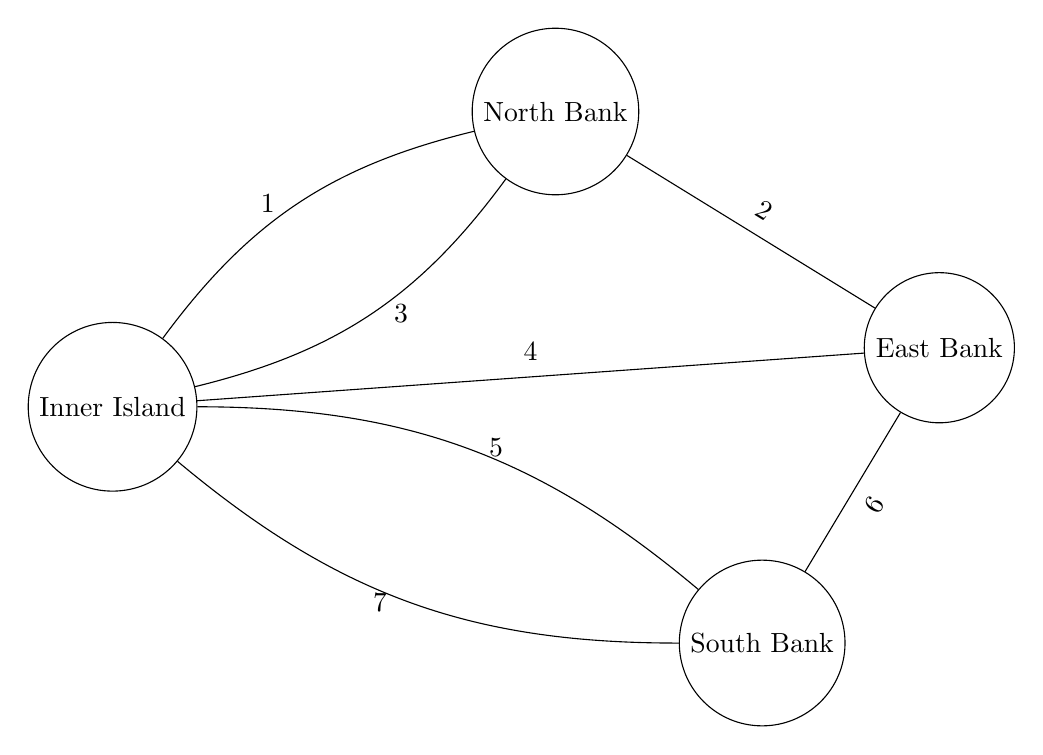
\begin{tikzpicture}[scale=1.5, every node/.style={circle, draw}]
                % Nodes
                \node (InnerIsland) at (-5, 0) {Inner Island};
                \node (NorthBank) at (-1.25, 2.5) {North Bank};
                \node (EastBank) at (2, 0.5) {East Bank};
                \node (SouthBank) at (0.5, -2) {South Bank};
            
                % Edges
% UPDATE THESE NUMBERS TO BE MORE RESENTATIVE OF FROM LEFT TO RIGHT, TOP TO BOTTOM
                % Inner Island to North Bank
                \draw (InnerIsland) to [bend right=20] node [midway, right, outer sep=2pt, draw=none] {3} (NorthBank);
                \draw (InnerIsland) to [bend left=20] node [midway, left, outer sep=2pt, draw=none] {1} (NorthBank);
                
                % Inner Island to East Bank
                \draw (InnerIsland) -- node [midway, above, draw=none] {4} (EastBank);
                
                % Inner Island to South Bank
                \draw (InnerIsland) to [bend right=20] node [midway, left, outer sep=2pt, draw=none] {7} (SouthBank);
                \draw (InnerIsland) to [bend left=20] node [midway, right, outer sep=2pt, draw=none] {5} (SouthBank);
                
                % North Bank to East Bank
                \draw (NorthBank) -- (EastBank) node [midway, above, sloped, draw=none] {2};
            
                % South Bank to East Bank
                \draw (SouthBank) -- (EastBank) node [midway, below, sloped, draw=none] {6};
            
            \end{tikzpicture}
            \caption{Illustration of the Königsberg Bridge Puzzle}
        \end{figure}

\newpage

\setcounter{theorem}{0}

% For some reason, the new package, Tikz
        \begin{theorem}
            (Handshake Theorem) The sum of the degrees is always twice the number of the edges.
        \end{theorem}   

        \vspace{\proofDistance}

        \begin{corollary}
            The sum of degrees is always even.
        \end{corollary}

        \begin{corollary}
            No graph has a single vertex of odd degree.
        \end{corollary}

        \vspace{\proofDistance}




        \subsubsection{Definitions}
        
            \begin{definition}
                A \textit{loop} is an edge which connects a vertex to itself.
            \end{definition}
    
            \begin{definition}
                Two vertices are \textit{adjacent} if there is an edge between them.
            \end{definition}
    
            \begin{definition}
                A \textit{path} is a sequence of adjacent vertices.*
            \end{definition}
             * Typically, edges are not used twice.
    
            \begin{definition}
                A \textit{circuit} is a path with the same initial starting and ending vertex.
            \end{definition}

            \begin{definition}
                A graph is \textit{connected} if each vertex can be reached by path from each other.
            \end{definition}

\newpage

%------------------------------------------------------------------------------

        \subsubsection{Directed Graph (Diagram)}

        \begin{figure}[h]
            \centering
            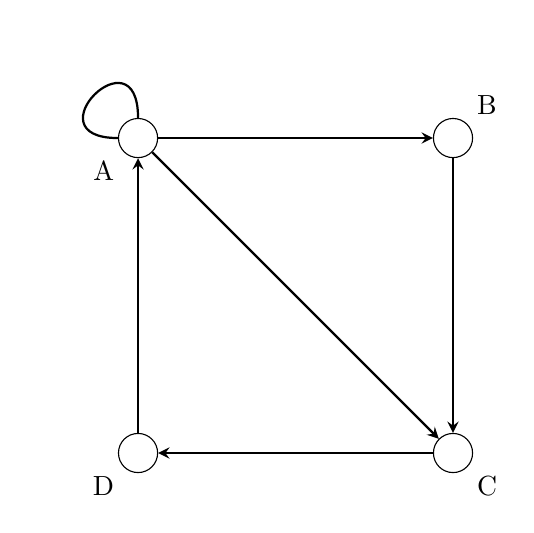
\begin{tikzpicture}[>=stealth] % Arrow tip style
                % Define corners of the rectangle with circles as vertices
                \node[draw, circle, fill=white, inner sep=5pt, label=below left:A] (A) at (0,0) {};
                \node[draw, circle, fill=white, inner sep=5pt, label=above right:B] (B) at (4,0) {};
                \node[draw, circle, fill=white, inner sep=5pt, label=below right:C] (C) at (4,-4) {};
                \node[draw, circle, fill=white, inner sep=5pt, label=below left:D] (D) at (0,-4) {};
                
                % Draw rectangle edges with arrows
                % \draw[parameters] (fromWhere) -- (toWhere);
                \draw[thick,->] (A) -- (B);
                \draw[thick,->] (B) -- (C);
                \draw[thick,->] (C) -- (D);
                \draw[thick,->] (D) -- (A);
                
                % Draw diagonal from A to C with arrow
                \draw[thick, ->] (A) -- (C);
        
                % Add loop from left to right on vertex A
                \draw[thick] (A) to [out=180,in=90,looseness=8] (A);
            \end{tikzpicture}
            \caption{Directed Graph pt. 1}
        \end{figure}


        \noindent in-degree: \\
        $A$ - 1, $B$ - 1, $C$ - 2, $D$ - 1

        \noindent out-degree: \\
        $A$ - 2, $B$ - 1, $C$ - 1, $D$ - 1

        

        \begin{figure}[h]
            \centering
            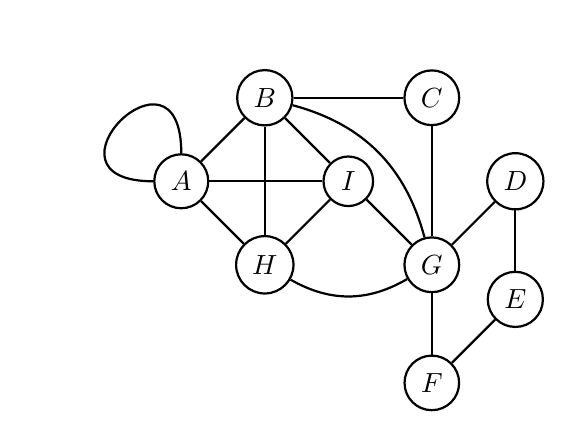
\begin{tikzpicture}[node distance={15mm}, thick, main/.style = {draw, circle, execute at begin node=$, execute at end node=$}]
                % Nodes
                \node[main] (A) {A};
                \node[main] (B) [above right of=A] {B};
                \node[main] (I) [below right of=B] {I};
                \node[main] (H) [below left of=I] {H};
                \node[main] (G) [below right of=I] {G};
                \node[main] (C) [above right of=I] {C};
                \node[main] (D) [above right of=G] {D};
                \node[main] (E) [below of=D] {E};
                \node[main] (F) [below of=G] {F};
                
                % Lines
                % \draw[parameters] (fromWhere) -- (toWhere);
                \draw (A) -- (B);
                \draw (A) -- (I);
                \draw (A) -- (H);
                \draw (B) -- (I);
                \draw (B) -- (C);
                \draw (B) -- (H);
                \draw (C) -- (G);
                \draw (D) -- (E);
                \draw (E) -- (F);
                \draw (F) -- (G);
                \draw (G) -- (D);
                \draw (G) -- (I);
                \draw (H) -- (I);
                
                \draw (B) to [bend left] (G);
                \draw (H) to [bend right] (G);
                
                \draw[thick] (A) to [out=180,in=90,looseness=8] (A);
            \end{tikzpicture}
            \caption{Social Network (Undirected Diagram)}
        \end{figure}
    
            \begin{figure}[htbp]
                \centering
                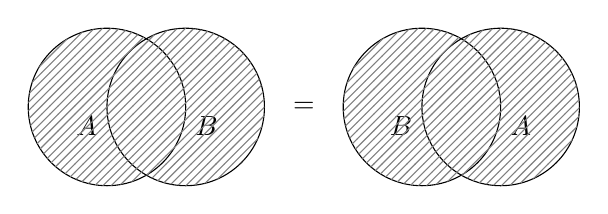
\begin{tikzpicture}
                    % Define the style for the diagonal lines pattern
                    \tikzstyle{diagonal lines}=[pattern=north east lines, pattern color=gray];
                    
                    % First pair of circles (A and B)
                    \coordinate (A1) at (1.5,1.5);
                    \coordinate (B1) at (2.5,1.5);
                    
                    % Draw first pair of circles for A and B
                    \draw (A1) circle (1cm) node [text=black,below left] {$A$};
                    \draw (B1) circle (1cm) node [text=black,below right] {$B$};
                    
                    % Fill the intersection of the first pair
                    \begin{scope}
                        \clip (A1) circle (1cm) (B1) circle (1cm);
                        \fill[diagonal lines] (-1,0) rectangle (5,3);
                    \end{scope}
                    
                    % Equals sign
                    \node at (4,1.5) {$=$};
                    
                    % Second pair of circles (B and A), switched positions
                    \coordinate (B2) at (5.5,1.5);
                    \coordinate (A2) at (6.5,1.5);
                    
                    % Draw second pair of circles for B and A
                    \draw (B2) circle (1cm) node [text=black,below left] {$B$};
                    \draw (A2) circle (1cm) node [text=black,below right] {$A$};
                    
                    % Fill the intersection of the second pair
                    \begin{scope}
                        \clip (B2) circle (1cm) (A2) circle (1cm);
                        \fill[diagonal lines] (3,0) rectangle (9,3);
                    \end{scope}
                    
                \end{tikzpicture}
                \caption{Demonstrating the commutative property of union, $A \cup B = B \cup A$, with sets $A$ and $B$ and their positions switched.}
            \end{figure}

\newpage
%------------------------------------------------------------------------------

    \subsection{Sets}

        \begin{definition}
            A \textit{set} is a collection of objects, called the \textit{elements}, or \textit{members}.
        \end{definition}

        \vspace{\subheaderSpace}

        We can list the elements like so: \\
        $\{1,2,3\}, \{5,10,21,23\}, \{1,3,\dots,5\}, \{1,3,5,\dots,11\}, \{1,3,5,7,\dots\}$
        
        \vspace{\subheaderSpace}

        \begin{terminology}
            Typically, sets are upper-case Latin: $A, B, X, Y, \dots$.
            Elements are lower-case Latin: $a,b,x,y,\dots$. \\
            And, if $a$ is an element of $X$, $a\in X$. Likewise, if $b$ is not in $X$, $b\notin X$.
        \end{terminology}

        \vspace{\subheaderSpace}

        \begin{definition}            
            There exists a set whose elements are exactly the elements of $A$ for which $s(x)$ is true.
            $\{x\in A\colon P(x)\}$ where $P$ is any predicate with $A$ as its domain. 
        \end{definition}

        \vspace{\subheaderSpace}

        \begin{example}
            $A = \{1,3,5,7,9\}$, then $\{x\in A\colon x^2 < 10\} = \{1,3\}$. This is called set builder notation. 
        \end{example}

        \vspace{\subheaderSpace}

        \begin{definition}
            The statement that set $A$ is \textit{equal} to set $B$ means $x\in A \iff x\in B$.
        \end{definition}

        \vspace{\subheaderSpace}

\setcounter{theorem}{1}

        \begin{theorem}
            Suppose $A,B,C$ are sets with $A=B$ and $B=C$. Then, $$A = C$$
        \end{theorem}

        \pf{
            Let $x\in A$. Since $A = B, x\in B$. \\
            \indent Since $B=C$, then $x\in C$. Now, let $y\in C$. Since $B=C, y\in B$. Since $A=B$ then $y\in A$. \\
            \indent Therefore, $A=C$
        }

        \vspace{\subheaderSpace}

        \begin{definition}
            Suppose $A$ and $B$ are sets. The statement that $A$ is a subset of $B$, denoted by $A\subseteq B$, means if $x\in A$, then $x\in B$
        \end{definition}

        \begin{figure}[htbp]
            \centering
            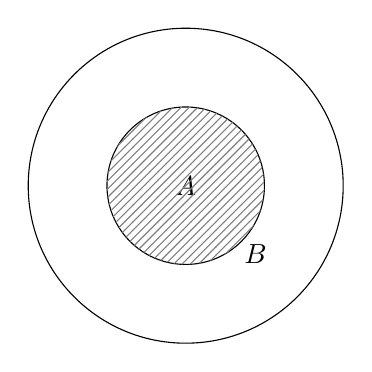
\begin{tikzpicture}
                % Define the style for the diagonal lines pattern
                \tikzstyle{diagonal lines}=[pattern=north east lines, pattern color=gray];
                
                % Coordinate for A
                \coordinate (A) at (2,2); 
                
                % Draw A 
                \draw (A) circle (1cm) node {$A$};
                
                % Draw B around A
                \draw (A) circle (2cm) node [below right=2.5em] {$B$};
                
                % Fill A to emphasize it is a subset of B
                \begin{scope}
                    \clip (A) circle (1cm);
                    \fill[diagonal lines] (0.5,0.5) rectangle (3.5,3.5);
                \end{scope}
                
            \end{tikzpicture}
            \caption{Set \( A \) as a subset of set \( B \).}
        \end{figure}



        \begin{theorem}
            Let $A$ be a set and $P$ a predicate. $\{x\in A\colon P(x)\}\subseteq A$.
        \end{theorem}

        \pf{
        Let $x\in \{x\in A\colon P(x)\}$. \\
        \indent By definition, $x\in A$. \\
        \indent Therefore, $x\in A$.
        }

        \vspace{\subheaderSpace}

        \begin{definition}
            The \textit{empty set}, (i.e., $\emptyset$, $\{\}$), the set with no elements: if $x$ exists, $x\notin \emptyset$.
        \end{definition}

        \vspace{\subheaderSpace}

\newpage

%------------------------------------------------------------------------------

        \begin{definition}
            Union and Intersection are defined as:
            \begin{itemize}
                \item Union: $A\cup B\colon x\in A\cup B$ if $x\in A$ or $x\in B$ 
                \item Intersection: $A\cap B\colon x\in A\cap B$ if $x\in A$ and $x\in B$.
            \end{itemize}
        \end{definition}

        \vspace{\subheaderSpace}

        \begin{figure}[htbp]
            \centering
            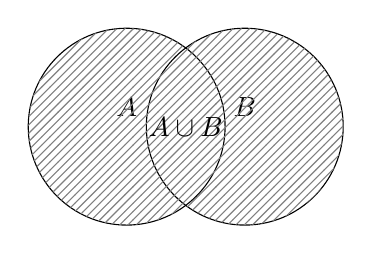
\begin{tikzpicture}
                % Define the style for the diagonal lines pattern
                \tikzstyle{diagonal lines}=[pattern=north east lines, pattern color=gray];
                
                % Define the coordinates for set A and B
                \coordinate (A) at (1.25,1.5);
                \coordinate (B) at (2.75,1.5);
                
                % Draw set A and set B with labels
                \draw (A) circle (1.25cm) node [text=black,above] {$A$};
                \draw (B) circle (1.25cm) node [text=black,above] {$B$};
                
                % Fill the union with diagonal lines
                \begin{scope}
                    \clip (A) circle (1.25cm) (B) circle (1.25cm);
                    \fill[diagonal lines] (0,0) rectangle (4,3);
                \end{scope}
        
                
                % Label the union
                \node at (2,1.5) {$A \cup B$};
            \end{tikzpicture}
            \caption{Venn diagram demonstrating the union of sets $A$ and $B$.}
        \end{figure}

        \begin{figure}[htbp]
            \centering
            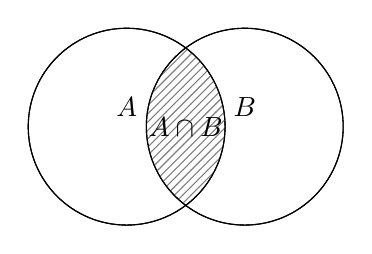
\begin{tikzpicture}
                % Define the style for the diagonal lines pattern
                \tikzstyle{diagonal lines}=[pattern=north east lines, pattern color=gray];
                
                % Define the coordinates for set A and B
                \coordinate (A) at (1.25,1.5);
                \coordinate (B) at (2.75,1.5);
                
                % Draw set A and set B without filling them
                \draw (A) circle (1.25cm) node [text=black,above] {$A$};
                \draw (B) circle (1.25cm) node [text=black,above] {$B$};
                
                % Fill the intersection (union) with diagonal lines
                \begin{scope}
                    \clip (A) circle (1.25cm);
                    \clip (B) circle (1.25cm);
                    \fill[diagonal lines] (1.5,1.5) circle (1.25cm);
                \end{scope}
                
                % Redraw the circles to bring the outlines to the front
                \draw (A) circle (1.25cm);
                \draw (B) circle (1.25cm);
                
                % Label the intersection
                \node at (2,1.5) {$A \cap B$};
            \end{tikzpicture}
            \caption{Venn diagram demonstrating the intersection of sets $A$ and $B$.}
        \end{figure}

        \vspace{\subheaderSpace}

        \begin{definition}
            Product: $A\times B$ is the set of all order pairs, $(a,b)$, where $a\in A, b\in B$. \\
            $A = \{1,2\}, B = \{2,4,6\}$ $A\times B = \{(1,2),(1,4),(1,6),(2,2),(2,4),(2,6)\}$
        \end{definition}

        \vspace{\subheaderSpace}

        \begin{definition}
            Suppose $A\subseteq U$. The \textit{complement} of $A$, relative to $U$ is $\{x\in U\colon x\notin A\} = A'$ (preferably, $\overline{A}$ or, $A^c$).
        \end{definition}

        \begin{figure}[htbp]
            \centering
            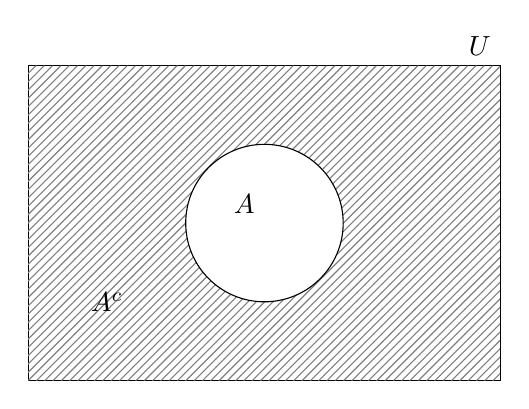
\begin{tikzpicture}
                \tikzstyle{diagonal lines}=[pattern=north east lines, pattern color=gray];
                % Define the rectangle for the universal set U
                \draw (0,0) rectangle (6,4) node[above left] {$U$};
                
                % Define the circle for set A without drawing it yet
                \coordinate (A) at (3,2);
                \coordinate (B) at (1,1);
                
                % Draw diagonal lines pattern in the rectangle excluding the circle
                \begin{scope}
                    \clip (0,0) rectangle (6,4) (A) circle (1cm);
                    \fill[diagonal lines] (0,0) rectangle (6,4);
                \end{scope}
                
                % Draw the circle for set A
                \draw (A) circle (1cm) node[above left] {$A$};
                \draw (B) node {$A^c$};
            \end{tikzpicture}
            \caption{Set diagram with $U$, set $A$, and its complement, $A^c$ (or $\overline{A}$), within $U$.}
        \end{figure}

\newpage

%------------------------------------------------------------------------------

        \begin{theorem}
            Let $A$ and $B$ be sets. Then, $$A\subseteq B \iff A\cap B = A$$
        \end{theorem}

        \pf{
        ($\Rightarrow$) \\
        Show that if $A\subseteq A\cap B = A$ \\
        
        \noindent Let $x\in A\cap B$. \\
        \indent Then, $x\in A$ and $x\in B$.
        \indent Therefore, $x\in A$. \\

        \noindent Let $y\in A$. \\
        \indent Since, $A\subseteq B$, $y\in B$. So, $y\in A$ and $y\in B$.

        \indent Therefore, $y\in A\cap B$. \\

        \noindent \textit{Proof.} ($\Leftarrow$) \\
        Show that $A\cap B = A$ then, $A\subseteq B$. \\

        \noindent Let $x\in A$. \\ 
        \indent Since $A = A\cap B$, $x\in A\cap B$. So, $x\in A$ and $x\in B$. \\
        \indent Therefore, $x\in B$.
        } 

\newpage

%------------------------------------------------------------------------------

    \subsection{Functions}

    \begin{definition}
        Let $X$ and $Y$ be sets. A \textit{function} $f$ is a well-defined rule that associates each element $x\in X$ with a unique $y\in Y$. We write this as $f(x)=y$.
    \end{definition}

    \vspace{5pt}

        $X$ Domain: \\
        $g\colon \R \rightarrow \R$ by $g(x) = \frac{1}{x-2}$. \\

        $Y$ Co-Domain: \\
        We require that $f$ is defined for each $x\in X$ (i.e., the domain). However, it is okay if not for each $y\in Y$ is matched. \\

        \begin{terminology}
            $f\colon X\rightarrow Y$ is a subset of $X\times Y$ so that each $x\in X$ belongs to exactly one pair.
        \end{terminology}

    \vspace{5pt}

    If $f\colon X\rightarrow X$ is a function, then this generates a directed graph: \\
    $X = \{0,1,2,3\}$. so, $f(0) = 1, f(1) = 3, f(2) = 1, f(3) = 3$ \\

        \begin{figure}[h]
            \centering
                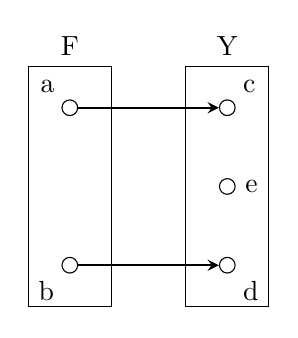
\begin{tikzpicture}[>=stealth] % Arrow tip style
                    % Define corners of the rectangle with circles as vertices
                    \node[draw, circle, fill=white, inner sep=2pt, label=above left:a] (A) at (0,0) {};
                    \node[draw, circle, fill=white, inner sep=2pt, label=above right:c] (C) at (2,0) {};
                    \node[draw, circle, fill=white, inner sep=2pt, label=below right:d] (D) at (2,-2) {};
                    \node[draw, circle, fill=white, inner sep=2pt, label=below left:b] (B) at (0,-2) {};
                    \node[draw, circle, fill=white, inner sep=2pt, label=right:e] (E) at (2,-1) {};
                    
                    % Draw rectangle edges with arrows
                    \draw[thick,->] (A) -- (C);
                    \draw[thick,->] (B) -- (D);
                
                    % Surround Nodes A and B with a box labeled F
                    \node[draw, rectangle, fit=(A) (B), inner sep=12pt, label=above:F] (BoxF) {};
                    
                    % Surround Nodes C and D with a box labeled Y
                    \node[draw, rectangle, fit=(C) (D), inner sep=12pt, label=above:Y] (BoxY) {};
                    
                \end{tikzpicture}
            \caption{Directed Graph of a Function}
        \end{figure}

\newpage

%------------------------------------------------------------------------------

        \begin{definition}
            Let $f\colon X \rightarrow Y$ be a function. we say $f$ is a \textit{one-to-one} or \textit{injective} if for each $x_1, x_2\in X$ if $f(x_1) = f(x_2)$, and $x_1 = x_2$.
        \end{definition}

        \setcounter{example}{0}

        \vspace{0.5cm}

        \begin{figure}[h]
            \centering
                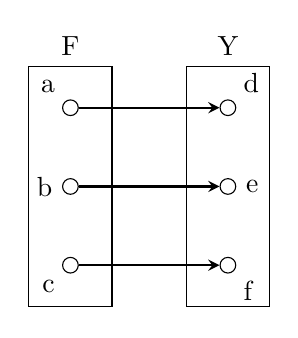
\begin{tikzpicture}[>=stealth] % Arrow tip style
                    % Define corners of the rectangle with circles as vertices
                    \node[draw, circle, fill=white, inner sep=2pt, label=above left:a] (A) at (0,0) {};
                    \node[draw, circle, fill=white, inner sep=2pt, label=left:b] (B) at (0,-1) {};
                    \node[draw, circle, fill=white, inner sep=2pt, label=below left:c] (C) at (0,-2) {};
                    \node[draw, circle, fill=white, inner sep=2pt, label=above right:d] (D) at (2,0) {};
                    \node[draw, circle, fill=white, inner sep=2pt, label=right:e] (E) at (2,-1) {};
                    \node[draw, circle, fill=white, inner sep=2pt, label=below right:f] (F) at (2,-2) {};

                    
                    % Draw rectangle edges with arrows
                    \draw[thick,->] (A) -- (D);
                    \draw[thick,->] (B) -- (E);
                    \draw[thick,->] (C) -- (F);
                
                    % Surround Nodes A and B with a box labeled F
                    \node[draw, rectangle, fit=(A) (C), inner sep=12pt, label=above:F] (BoxF) {};
                    
                    % Surround Nodes C and D with a box labeled Y
                    \node[draw, rectangle, fit=(D) (F), inner sep=12pt, label=above:Y] (BoxY) {};
                    
                \end{tikzpicture}
            \caption{Directed Graph of an One-To-One Function}
        \end{figure}

        \vspace{0.5cm}

        \begin{example}
            Let $f\colon \N \rightarrow \N$ by $f(n) = 3n + 1$. Then, $f$ is one-to-one.
        \end{example}

        \pf{
            Let $x_1,x_2\in \N$ so that $f(x_1) = f(x_2)$. We hope to show $x_1 = x_2$. \\

            $f(x_1) = 3x_1 + 1$ and $f(x_2) = 3x_2 + 1$. Then, 
            \begin{align*}
                3x_1 + 1 &= 3x_2 + 1 \\
                3x_1 &= 3x_2 \\
                x_1 &= x_2 \\
            \end{align*}

            Therefore, $f$ is one-to-one.
        }

        \begin{example}
            Let $f\colon \Z \rightarrow \Z$ by $f(z) = z^2 - 3$. $f$ is not one-to-one. Find $x_1 \ne x_2$ so that $f(x_1) = f(x_2)$. 
        \end{example}

        \begin{solution}
            consider $x_1 = 2, x_2 = -2$. Since $x_1 \ne x_2$, but $f(x_1) = 1 = f(x_2)$, $f$ is not one-to-one.
        \end{solution}

        \proofseparator

        \vspace{0.5cm}

        \begin{example}
            Let $f\colon \N \rightarrow \N$ by $f(x) = \frac{n}{n} = 1$.
        \end{example}

        \begin{solution}
            Consider $n_1 = 2, n_2 = 3. f(n_1) = 1 = f(n_2)$.
        \end{solution}

        \proofseparator

        \begin{definition}
            $f\colon X\rightarrow Y$ is \textit{onto} or \textit{surjective}. If for-each $y\in Y$. there exists at least one $x\in X$ so that $f(x) = y$.
        \end{definition}

        \vspace{0.5cm}

        \begin{figure}[h]
            \centering
                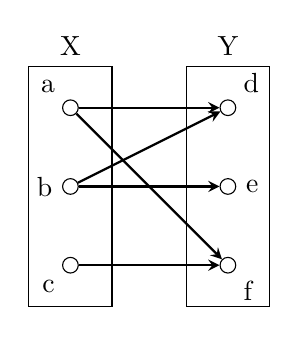
\begin{tikzpicture}[>=stealth] % Arrow tip style
                    % Define corners of the rectangle with circles as vertices
                    \node[draw, circle, fill=white, inner sep=2pt, label=above left:a] (A) at (0,0) {};
                    \node[draw, circle, fill=white, inner sep=2pt, label=left:b] (B) at (0,-1) {};
                    \node[draw, circle, fill=white, inner sep=2pt, label=below left:c] (C) at (0,-2) {};
                    \node[draw, circle, fill=white, inner sep=2pt, label=above right:d] (D) at (2,0) {};
                    \node[draw, circle, fill=white, inner sep=2pt, label=right:e] (E) at (2,-1) {};
                    \node[draw, circle, fill=white, inner sep=2pt, label=below right:f] (F) at (2,-2) {};

                    
                    % Draw rectangle edges with arrows
                    \draw[thick,->] (A) -- (D);
                    \draw[thick,->] (A) -- (F);
                    \draw[thick,->] (B) -- (D);
                    \draw[thick,->] (B) -- (E);
                    \draw[thick,->] (C) -- (F);
                
                    % Surround Nodes A and B with a box labeled F
                    \node[draw, rectangle, fit=(A) (C), inner sep=12pt, label=above:X] (BoxF) {};
                    
                    % Surround Nodes C and D with a box labeled Y
                    \node[draw, rectangle, fit=(D) (F), inner sep=12pt, label=above:Y] (BoxY) {};
                    
                \end{tikzpicture}
            \caption{Directed Graph of an Onto Function}
        \end{figure}

        \vspace{0.5cm}
        
        \begin{example}
            $f\colon \N \rightarrow \N$ by $f(n) = n^2$ is not onto. 
        \end{example}

        \begin{solution}
            Consider $2\in \N$ (the co-domain). there is no $n\in \N$ for which $n^2=2$.
        \end{solution}

        \proofseparator

        \begin{example}
            $g\colon \N\rightarrow \N$ by $g(n) = |n-1| + 1$ is onto.
        \end{example}

        \begin{solution}
            Show $g$ is onto: Let $y\in \N$. Goal: Find $n$ so that $g(n)=y$. Consider $y\in \N$. Then, $g(y) = |y-1| + 1$. Since $y\geq 1, |y-1| = y -1,$ so $g(y) = y - 1 + 1 = y$. 
        \end{solution}

        \proofseparator

        \begin{example}
             Show $h$ is onto: $h(n) = |n-7| + 1$
        \end{example}

        \begin{solution}
            Let $y\in \N$. Consider $y + 6\in \N$. Then, $(y + 6) \in \N$. Then, $(y + 6) \geq 0$, so $|(y+6) - 7| = (y+ 6) - 7$. Then, $h(y) = |y+6-7| + 1 = y +6-7+1 = y$.
        \end{solution}

        \proofseparator

        \begin{example}
            Suppose $f\colon X\rightarrow Y$ is one-to-one. Then we can define $f^{-1}$ by $f^{-1}(y) =x \iff f(x)=y$
        \end{example}

        \begin{solution}
            $f\colon \R$ by $f(x) = x^2$ does \textit{not} have an inverse. $g\colon [0,\infty) \rightarrow [0, \infty)$ by $g(x) = x^2$ \textit{does} have an inverse: $g^{-1}(x)=\sqrt{x}$.
        \end{solution}

        \proofseparator

        \begin{example}
            Suppose $f\colon X\rightarrow Y$ and $g\colon Y\rightarrow Z$ are functions that we define as $h = g \circ f$ by $h(x) = g(f(x))$ so $h\colon X\rightarrow Z$.
        \end{example}

    \subsection{Relations}

        \begin{definition}
            A \textit{relation} is a generalization of the idea of a function. 
            Thus, $$R\colon X\rightarrow Y \text{ is a relation if } R\subseteq X\times Y.$$
        \end{definition}
        \textbf{Note}: All Functions are Relations, but not all Relations are Functions. \\
        If an $x$ value can be mapped to more than one $y$ value, the statement is not a function. \\

        \begin{example}
            For the given relation, is it a function? Consider the relation $R \colon \R\rightarrow \R$, such that $R := \{\{2,3\}, \{4,3\}, \{3,4\}, \{2,8\}\}$.
        \end{example}
        \noindent This is not a function because an $x$-value, $2$, is mapped to multiple $y$-values. 

        \vspace{0.5cm}

        \begin{terminology}
            $$R = \{( \ , \ ), ( \ , \ ), ( \ , \ )\}$$
        \end{terminology}

        Assume both $p$ and $\neg p$ are true and let $q$ be a statement.
        \begin{table}[htb]
            \centering
            \renewcommand{\arraystretch}{0.8} % Reduce row spacing
                \begin{tabular}{@{}c@{\hspace{2mm}}c@{\hspace{2mm}}l@{}} % Adjusted column spacing
                    $<$ & $\colon$ & $\N \rightarrow \N$ \\
                    $<$ & $=$ & $\{(1,2), (1,3), (1,4), \dots,$ \\
                       &   & $(2,3), (2,4), (2,5), \dots,$ \\
                       &   & $(3,4), (3,5), (3,6), \dots,$ \\
                       &   & $\dots \}$ \\
                \end{tabular}    
        \end{table}
    
        
        \begin{example}
            $X, Y = $ set of Hendrix Students: $a \ R \ b$ if $a$ has taken a class with $b$.
        \end{example}

        \vspace{0.5cm}
        
        \begin{definition}    
            If $R\colon X\rightarrow X$ is a relation, we say that $R$ is:
            \begin{itemize}
                \item \textit{Reflexive} if for each $x\in X$, $x \ R \ x$.
                \item \textit{Symmetric} if when $a \ R \ b$, then $a\ R \ b$.
                \item \textit{Transitive} if when $a \ R \ b$, and $b \ R \ c$, then $a \ R \ c$.
            \end{itemize}
        \end{definition}
        \textbf{Note}: There exists relations that can be none, one, two, or all of the previous traits. 

        \begin{definition}
            If it a relation is satisfies all three traits, then it is called an \textit{equivalence relation}.
        \end{definition}
        \textbf{Note}: This allows us to \textit{partition} a domain.

        \begin{definition}
            Each partition is called an \textit{equivalence class}. Denoted as $[a]$.
        \end{definition}

        \vspace{0.5cm}

        \begin{example}
            Let $a,b \in \N$ and say $a \ R \ b$. Such that if $a$ divides into $b$.
            \begin{itemize}
                \item $3 \ R \ 12$
                \item $7 \ R \ 49$
                \item $5 \ \slashed{R} \ 12$
            \end{itemize}
        \end{example}
        
        \noindent $R$ is reflexive. Let $a\in \N$. $a$ is divisible by $a$, so $a \ R \ a$. \\
        $R$ is not symmetric. Consider $7 \ R \ 49$, but $49  \ \slashed{R} \ 4$. \\
% Add align for transitivity along the equals sign
        $R$ is transitive. Consider $a \ R \ b$, and $b \ R \ c$. \\
        Then, $a\cdot k$, and $c = b\cdot l$ for some $k, l$. \\
        Then, $c = b\cdot l$ \\
        $c = (a\cdot k)\cdot l$ \\
        $c = a\cdot (k \cdot l)$

        \vspace{0.5cm}

        \begin{example}
            If [a] is a set (in fact, a subset of $X$), then $a\in [a]$ if: 
            \begin{itemize}
                \item $b\in [a]$, then $a\in [b]$. $a \ R \ b \Rightarrow [a] = [b]$.
                \item $a\in [b], b\in [c], a\in [c]$.
            \end{itemize}
        \end{example}

        \subsubsection{Modular Arithmetic}
            \begin{definition}
                Let $n\in \N.$ Let $a,b\in \Z.$ \\
                We say $a$ is \textit{equivalent to} $b$, modulo ($\%$), $a \equiv b \mod{n}$, if $(a-b)$ is divisible by $n$.
            \end{definition}
        
            \begin{itemize}
                \item Is $a \equiv a \mod{n}$ reflexive? Yes. \\
                $a - a = 0$ which is certainly divisible by $n$.
                \item Is $a \equiv a \mod{n}$ symmetric? Yes. \\
                If $a\equiv b\mod{n}$ is $b\equiv a\mod{n}$? \\
                $(a-b)$ is divisible by $n$. Well, $b-a$ is also divisible by $n$.
                \item Is $a \equiv a \mod{n}$ transitive? Yes. \\
                $a\equiv b\mod{n}$, and $b\equiv c \mod{n}$, is $a \equiv c \mod{n}$? \\
            \end{itemize}

\newpage

%------------------------------------------------------------------------------

\setcounter{subsection}{5}
    \subsection{Graph Theory}
        \subsubsection{Graphs}

            \begin{definition}
                A \textit{graph} $G=(V,E)$, is a pair of sets $V,$ the \textit{vertex set}, and $E$, the $edge set$, so that each element of $E$ has the form $\{v_i,v_j\}, v_i,v_j \in V$.
            \end{definition}
        
                \begin{figure}[h]
                    \centering
                    \begin{tikzpicture}[>=stealth] % Arrow tip style
                        % Define corners of the rectangle with circles as vertices
                        \node[draw, circle, fill=white, inner sep=5pt, label=above left:A] (A) at (0,0) {};
                        \node[draw, circle, fill=white, inner sep=5pt, label=above right:B] (B) at (4,0) {};
                        \node[draw, circle, fill=white, inner sep=5pt, label=below right:C] (C) at (4,-4) {};
                        \node[draw, circle, fill=white, inner sep=5pt, label=below left:D] (D) at (0,-4) {};
                        
                        % Draw rectangle edges with arrows
                        % \draw[parameters] (fromWhere) -- (toWhere);
                        \draw (A) -- (B);
                        \draw (B) -- (C);
                        \draw (D) -- (A);
                        
                        % Draw diagonal from A to C with arrow
                        \draw (A) -- (C);
        
                    \end{tikzpicture}
                    \caption{Graph with vertices and edges.}
                \end{figure}
        
            \noindent $G\colon \\
            V = \{a,b,c,d\}, \\
            E = \{\{a,b\},\{a,c\},\{a,d\},\{b,c\}\}$ \\
        
            \begin{definition}
                Given $v\in V$, the \textit{degree} of $v$ (denoted as $\deg(v)$) is the number of edges which include $v$.
            \end{definition} 
    
            \begin{definition}
                We say vertex $u$ is \textit{adjacent} to vertex $v$ if, and only if, $\{u, v\} \in E$. 
            \end{definition}
            \textbf{Note}: For us, no vertex is adjacent to itself because we are ignoring graphs that have loops.
    
            \vspace{0.5cm}
    
            \begin{definition}
                A \textit{path} from vertex $v_0$ to vertex $v_n$ is a sequence $v_0, v_1, v_2, \dots, v_n$, where each $v_i\in V$ and $\{v_i,v_{i+1}\} \in E$. 
            \end{definition}
    
            \begin{definition}
                A path is \textit{simple} if no edge occurs twice.
            \end{definition}
    
            \begin{definition}
                 Two vertices are \textit{connected} if there is a path (edge) from one to the other. In other words, a graph is connected if each pair of vertices are connected.
            \end{definition}

\newpage
%------------------------------------------------------------------------------

        \subsubsection{Circuits}

            \begin{definition}
                A \textit{circuit} is a path with the same starting and ending vertex.
            \end{definition}
    
            \begin{definition}
                The \textit{complete graph} on $n$ vertices, $K_n$, is the connected graph where each vertex is adjacent to each other.
            \end{definition}
    
            \vspace{1.0cm}
    
            \begin{figure}[h]
                \begin{subfigure}{}
                    \centering
                    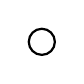
\begin{tikzpicture}[node distance={15mm}, thick, main/.style = {draw, circle, execute at begin node=$, execute at end node=$}]
                        \node[main] (A) {};
                    \end{tikzpicture}
                    \caption{$k_1$ (just a single vertex)}
                \end{subfigure}
                
                \vspace{0.6cm}
                
                \begin{subfigure}{}
                    \centering
                    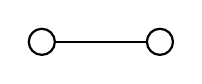
\begin{tikzpicture}[node distance={15mm}, thick, main/.style = {draw, circle, execute at begin node=$, execute at end node=$}]
                        \node[main] (A) {};
                        \node[main] (B) [right of=A] {};
                        \draw (A) -- (B);
                    \end{tikzpicture}
                    \caption{$k_2$ (two vertices and an edge)}
                \end{subfigure}
                
                \vspace{0.6cm}
            
                \begin{subfigure}{}
                    \centering
                    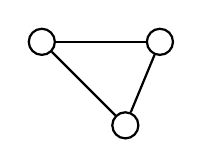
\begin{tikzpicture}[node distance={15mm}, thick, main/.style = {draw, circle, execute at begin node=$, execute at end node=$}]
                        \node[main] (A) {};
                        \node[main] (B) [right of=A] {};
                        \node[main] (C) [below right of=A] {};
                        \draw (A) -- (B);
                        \draw (A) -- (C);
                        \draw (B) -- (C);
                    \end{tikzpicture}
                    \caption{$k_3$ (three vertices and three edges)}
                \end{subfigure}
            
                \vspace{0.6cm}
            
                \begin{subfigure}{}
                    \centering
                    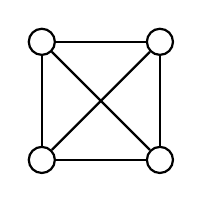
\begin{tikzpicture}[node distance={15mm}, thick, main/.style = {draw, circle, execute at begin node=$, execute at end node=$}]
                        \node[main] (A) {};
                        \node[main] (B) [right of=A] {};
                        \node[main] (C) [below of=A] {};
                        \node[main] (D) [below of=B] {};
                        \draw (A) -- (B);
                        \draw (A) -- (C);
                        \draw (A) -- (D);
                        \draw (B) -- (C);
                        \draw (B) -- (D);
                        \draw (C) -- (D);
                    \end{tikzpicture}
                    \caption{$k_4$ (four vertices and six edges)}
                \end{subfigure}
            \end{figure}


\newpage
%------------------------------------------------------------------------------

        \subsubsection{Bipartite}

            \begin{definition}
                A graph is \textit{bipartite} if the vertex set $V = v_1 \cup v_2$, $v_1\cap v_2 = \emptyset$, and no vertex in $V_1$ is adjacent to any other in $V_1$ and no vertex in $V_2$ is adjacent to any other in $V_2$.
            \end{definition}
    
            \begin{figure}[h]
                \centering
                    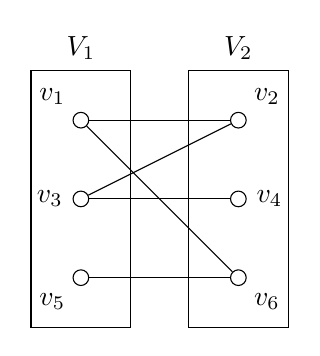
\begin{tikzpicture}[>=stealth] % Arrow tip style
                        % Define corners of the rectangle with circles as vertices
                        \node[draw, circle, fill=white, inner sep=2pt, label=above left:$v_1$] (A) at (0,0) {};
                        \node[draw, circle, fill=white, inner sep=2pt, label=left:$v_3$] (B) at (0,-1) {};
                        \node[draw, circle, fill=white, inner sep=2pt, label=below left:$v_5$] (C) at (0,-2) {};
                        \node[draw, circle, fill=white, inner sep=2pt, label=above right:$v_2$] (D) at (2,0) {};
                        \node[draw, circle, fill=white, inner sep=2pt, label=right:$v_4$] (E) at (2,-1) {};
                        \node[draw, circle, fill=white, inner sep=2pt, label=below right:$v_6$] (F) at (2,-2) {};
    
                        
                        % Draw rectangle edges with arrows
                        \draw (A) -- (D);
                        \draw (A) -- (F);
                        \draw (B) -- (D);
                        \draw (B) -- (E);
                        \draw (C) -- (F);
    
                        \node[draw, rectangle, fit=(A) (B) (C), inner sep=15pt, label=above:$V_1$] (BoxV) {};
                        
                        \node[draw, rectangle, fit=(D) (E) (F), inner sep=15pt, label=above:$V_2$] (BoxY) {};
                        
                        
                    \end{tikzpicture}
                \caption{Bipartite Graph}
            \end{figure}

\vspace{3cm}
%------------------------------------------------------------------------------

        \subsubsection{Trees}

            \begin{definition}
                A graph is \textit{tree} if it is connected and has no circuit.
            \end{definition}
    
            \begin{figure}[h]
                \centering
                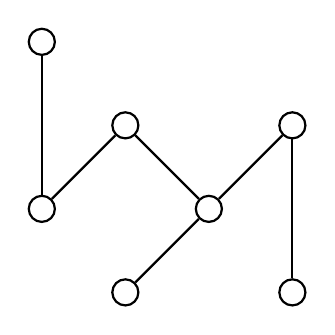
\begin{tikzpicture}[>=stealth, node distance={15mm}, thick, main/.style = {draw, circle}][>=stealth] 
                
                    \node[main] (1) {}; 
                    \node[main] (2) [above right of=1] {}; 
                    \node[main] (3) [below right of=1] {}; 
                    \node[main] (4) [above right of=3] {}; 
                    \node[main] (5) [above right of=4] {}; 
                    \node[main] (6) [below right of=4] {}; 
                    \node[main] (7) [above left of= 2] {};
                    
                    \draw (1) -- (2); 
                    \draw (2) -- (4); 
                    \draw (3) -- (4); 
                    \draw (5) -- (4); 
                    \draw (6) -- (5); 
                    \draw (7) -- (1);
                \end{tikzpicture} 
                \caption{Tree}
            \end{figure}

\newpage
%------------------------------------------------------------------------------


            \begin{figure}[htbp]
                \centering
                \begin{tikzpicture}[level/.style={sibling distance=60mm/#1}]
                    \node [circle, draw] (z){$8$}
                    child {node [circle, draw] (a) {$3$}
                        child {node [circle, draw] (b) {$1$}}
                        child {node [circle, draw] (c) {$6$}
                            child {node [circle, draw] (d) {$4$}}
                            child {node [circle, draw] (e) {$7$}}
                        }
                    }
                    child {node [circle, draw] (f) {$10$}
                        child {node [circle] {$\quad$} edge from parent[draw=none]} % null drawings to align tree placement
                        child {node [circle, draw] {$14$}
                            child {node [circle, draw] {$13$}}
                            child {node [circle] {$\quad$} edge from parent[draw=none]} % null drawings to align the tree placement
                        }
                    };
                \end{tikzpicture}
    
                \caption{Binary Search Tree}
    
            \end{figure}

            \vspace{0.5cm}

            \begin{lemma}
                If $G$ is a tree, $G$ has at least one vertex of degree 1. 
            \end{lemma}

            \pf{
                For the sake of contradiction, suppose each vertex has degree $\geq 2$. Pick a vertex, $v_0$. Since, $\deg(v_0) \geq 2$, it is adjacent to some $v_j$. Because $\deg(v_1) \geq 2$, it has an edge distinct from $\{v_0,v_1\}$, follow it to $v_2$. Then, $v_2$ has edge distinct from $\{v_1,v_2\}$, follow it to $v-3$. If $v_3=v_0 (v_1,v_2)$ we have a circuit. $v_3$ has edge distinct from $\{v_2,v_3\}$. Go to $v_4$. Continue \dots. Either some $v_j$ is visited again, or $v_0,v_1,v_2,\dots v_n$. Therefore, it must be a circuit. \\

                Hence, $G$ must have a vertex with degree of at least 1 such that $1\leq$.
            }

\setcounter{theorem}{0}
            
            \begin{theorem}
                A tree with $n$ vertices always has $n-1$ edges.
            \end{theorem}

            \pf{
                By the Lemma, there exists a vertex of degree 1. Remove it and its edge. We still have a tree. This new tree has vertex of degree 1. Remove it and its edge. Continue until you get to $k_2$, then $k_1$. We stop with 1 vertex, 0 edges, we have removed $n-1$ vertices. Each edge was removed. \\

                Thus, we threw out \textit{all} $n-1$ edges.
            }



            

\newpage
%------------------------------------------------------------------------------

        \subsubsection{Euler Circuit}

            \begin{definition}
                A graph has an \textit{Euler circuit} if there is a circuit which uses each edge only once. Similarly, an \textit{Euler path} is a path which uses each edge -- start and end vertices are distinct.
            \end{definition}
    
            \noindent \textbf{Notes}: $G$ has an Euler circuit if, and only if, it is connected and each vertex has an even degree. Intuitively, if each vertex has an even degree, then if you come into the vertex through the entrance (first edge), and you leave through the exit (second edge) you have used up both openings. \\
    
            $G$ has an Euler path if, and only if, it is connected and has exactly two vertices of odd degree. 
    
            \begin{figure}[h]
                \centering
                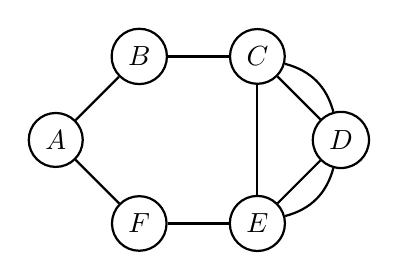
\begin{tikzpicture}[node distance={15mm}, thick, main/.style = {draw, circle, execute at begin node=$, execute at end node=$}]
                    % Nodes
                    \node[main] (A) {A};
                    \node[main] (B) [above right of=A] {B};
                    \node[main] (C) [right of=B] {C};
                    \node[main] (D) [below right of=C] {D};
                    \node[main] (E) [below left of=D] {E};
                    \node[main] (F) [below right of=A] {F};
                    
                    % Lines
                    % \draw[parameters] (fromWhere) -- (toWhere);
                    \draw (A) -- (B);
                    \draw (A) -- (F);
                    \draw (B) -- (C);
                    \draw (C) -- (D);
                    \draw (C) -- (E);
                    \draw (E) -- (D);
                    \draw (E) -- (F);
        
                    
                    \draw (C) to [bend left] (D);
                    \draw (E) to [bend right] (D);
                \end{tikzpicture}
                \caption{Euler Circuit}
            \end{figure}
    
            \centerline{For this to be an Euler path, simply remove the line that connects $C$ to $E$.}

\vspace{3.5cm}
%------------------------------------------------------------------------------

        \subsubsection{Isomorphism}
            \begin{definition}
                Two graphs, $G = (V,E)$ and $H = (W,f)$ are \textit{isomorphic} if $\exists f\colon V\rightarrow W$ which is one-to-one, onto, and $\{v_i, v_j\} \in E \iff \{f(v_i), f(v_j)\} \in F$.
            \end{definition}


\newpage
%------------------------------------------------------------------------------

        \subsubsection{Vertex Colorings}

            \begin{definition}
                Given a graph $G$, assign a color to each vertex so that two adjacent vertices have different colors.
            \end{definition}

            \noindent If $G$ contains a triangle (i.e., if it has a copy of $k_3$), we need at least 3. In $G$ contains a copy of $K_n$, we need at least $n$. \\

            If a graph has no overlapping paths, the graph requires no more than 4 colors.

            \hfill

            \begin{figure}[htpb]
                \centering
                
                % First subfigure
                \begin{subfigure}[]{}
                    \centering
                    \begin{tikzpicture}[scale=1.5, auto,swap]
                        % Define vertices with colors
                        \foreach \pos/\name/\color in {{(0,2)/a/red}, {(2,2)/b/green}, {(1,1)/c/blue}}
                            \node[vertex, fill=\color!50] (\name) at \pos {$\name$};
                        
                        % Connect vertices with edges
                        \foreach \source/ \dest in {a/b, a/c, b/c}
                            \path[edge] (\source) -- (\dest);
                    \end{tikzpicture}
                \end{subfigure}
                
                \hfill
                
                % Second subfigure
                \begin{subfigure}[]{}
                    \centering
                    \begin{tikzpicture}[scale=1.5, auto,swap]
                        % Square vertices
                        \foreach \pos/\name/\color in {{(4,2)/d/orange}, {(5,2)/c/blue}, {(5,3)/b/green}, {(4,3)/a/red}}
                            \node[vertex, fill=\color!50] (\name) at \pos {$\name$};
                        
                        % Square edges
                        \foreach \source/ \dest in {a/b, a/d, b/c, d/c, a/c, d/b}
                            \path[edge] (\source) -- (\dest);
                    \end{tikzpicture}
                \end{subfigure}
                
                \hfill
                
                % Third subfigure
                \begin{subfigure}[]{}
                    \centering
                    \begin{tikzpicture}[scale=1.5, auto,swap]
                        % Pentagon vertices
                        \foreach \pos/\name/\color in {{(0.9,0)/e/yellow}, {(2.3,0)/d/orange}, {(2.7,1.0)/c/blue}, {(1.6,1.6)/b/green}, {(0.5,1.0)/a/red}}
                            \node[vertex, fill=\color!50] (\name) at \pos {$\name$};
                        
                        % Pentagon edges
                        \foreach \source/ \dest in {e/d, d/c, c/b, b/a, a/e, a/c, a/d, b/d, b/e, c/e, c/a, d/a, d/b}
                            \path[edge] (\source) -- (\dest);
                    \end{tikzpicture}
                \end{subfigure}
                
                \hfill

                % Fourth subfigure
                \begin{subfigure}[]{}
                    \centering
                    \begin{tikzpicture}[scale=1.5, auto,swap]
                    

                        % Define the vertices with their color
                        \foreach \pos/\name/\color in {
                            {(0,0)/a/red}, {(1,1)/b/green}, {(1,0)/c/red},
                            {(1,-1)/d/blue}, {(2,1)/e/blue}, {(2,0)/f/red},
                            {(2,-1)/g/green}, {(3,0)/h/red}, {(3,-1)/i/blue}}
                            \node[vertex, fill=\color!50] (\name) at \pos {$\name$};
            
                        % Connect vertices with edges
                        \foreach \source/ \dest in {a/b, a/d, a/g, b/e, b/c, c/i, c/d, d/f, d/g, i/h}
                            \path[edge] (\source) -- (\dest);
            
                    \end{tikzpicture}
                \end{subfigure}
                \caption{Vertex Colorings}
                
            \end{figure}
            
\newpage 

%------------------------------------------------------------------------------

        \subsubsection{Hamilton Graphs}

            \begin{definition}
                A graph has a \textit{Hamilton Circuit} if there is a circuit that uses each vertex once. 
            \end{definition}
            \textbf{Notes}: \\
            This is different from Euler, as Euler uses edges. This is specifically for vertices. \\
            If it has a vertex of degree 1, it cannot have a Hamilton circuit.

            \vspace{0.5cm}

            \begin{figure}[h]
            \centering
            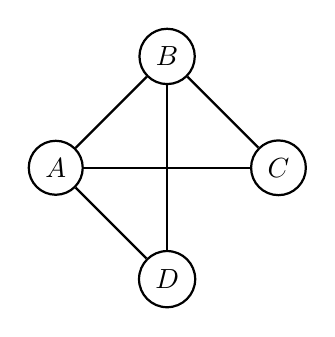
\begin{tikzpicture}[node distance={20mm}, thick, main/.style = {draw, circle, execute at begin node=$, execute at end node=$}]
                % Nodes
                \node[main] (A) {A};
                \node[main] (B) [above right of=A] {B};
                \node[main] (C) [below right of=B] {C};
                \node[main] (D) [below left of=C] {D};
                
                % Lines
                % \draw[parameters] (fromWhere) -- (toWhere);
                \draw (A) -- (B);
                \draw (A) -- (C);
                \draw (A) -- (D);
                \draw (B) -- (D);
                \draw (B) -- (C);
                
                
            \end{tikzpicture}
            \caption{Hamilton Circuit}
        \end{figure}

\newpage
%------------------------------------------------------------------------------

\section{Recursive Thinking}

    \subsection{Recurrence Relations}

        \[
        A(n) = 
        \begin{cases} 
            1 & \text{if } n = 1 \\
            A(n-1) + n & \text{if } n > 1
        \end{cases}
        \]

        Where $A(n) = 1$ is the base case, and $A(n) = A(n -1) + n)$ is the recursive case.

        For example, consider $A(2)$

        \begin{align*}
            A(2) &= A(2-1)+ 2 \\
            &= A(1) + 2 \\
            &= 1 + 2 \\
            &= 3 \\
        \end{align*}

        \begin{table}[h]
            \centering
            \begin{tabular}{c|c}
                $n$ & $A(n)$ \\
                \hline
                1 & 1 \\
                2 & 3 \\
                3 & 6 \\
                4 & 10 \\
                5 & 15 \\
                6 & 21 \\
                7 & 28
            \end{tabular}
            \caption{$A(n)$ Bottom Up}
            \label{Bottom Up A(n)}
        \end{table}

        \begin{table}[h]
            \centering
            \begin{align*}
                A(7) &= A(6) + 7 \\
                &= A(5) +6 + 7 \\
                &= A(4) + 5 + 6 + 7 \\
                &\ \ \ \ \ \ \ \ \ \ \ \ \ \ \ \vdots \\
                &= A(1) + 2 + 3 + 4 + 5 + 6 + 7
            \end{align*}
            \caption{$A(n)$ Top Down}
            \label{Top Down A(n)}
        \end{table}

        What about $A(100)$? We would use $\frac{n(n+1)}{2}$. We can always do bottom-up or top-down, but it might be tedious. Can we find and prove closed form explicit expression?

\newpage
%------------------------------------------------------------------------------

        $S\colon \N \rightarrow \N$ by: 
        $S(n) =$$
        \begin{cases} 
            1 & \text{if } n = 1 \\
            A(n-1) + 2n - 1 & \text{if } n > 1
        \end{cases} $ \\
        
        This can be modelled like $S(n) = n^2$. \\

        \vspace{0.3cm}

        $f\colon \N \rightarrow \N$ by:
        $f(n) =$$
        \begin{cases} 
            1 & \text{if } n = 0 \\
            n \cdot f(n-1) & \text{if } n > 0
        \end{cases} $ \\

        This can be modelled like $f(n) = n!$.

        \vspace{0.3cm}

        \subsubsection{Fibonacci}

            Start with a pair of rabbits in month 1. After 2 total months, any rabbit pair makes a new pair. This can be modelled with the piece-wise function below: \\

            $F\colon \R \rightarrow \R$ by: 
            $F(n) =
            \begin{cases} 
                1 & \text{if } n = 1 \text{ or } n = 2 \\
                F(n-1) + F(n-2) & \text{if } n > 2
            \end{cases} $ \\
            
            \begin{table}[h]
                \centering
                \begin{tabular}{c|c}
                    $n$ & $F(n)$ \\
                    \hline
                    1 & 1 \\
                    2 & 1 \\
                    3 & 2 \\
                    4 & 3 \\
                    5 & 5 \\
                    6 & 8 \\
                    7 & 13
                \end{tabular}
                \caption{Fibonacci Bottom Up}
                \label{Bottom Up}
            \end{table}

            \begin{table}[h]
                \centering
                \begin{align*}
                    F(7) &= F(6) + F(5) \\
                    &= F(5) = F(4) + F(4) + F(3)\\
                    &= A(4) + 5 + 6 + 7 \\
                    &= \ \vdots \\
                    &= F(1) + F(2) + 11 \\
                    & = 13
                \end{align*}
                \caption{Fibonacci Top Down}
                \label{Top Down Fibonacci}
            \end{table}

\newpage
%------------------------------------------------------------------------------

    \subsection{Mathematical Induction}
        \setcounter{example}{0}
        \begin{example}
            Suppose we want to prove some logical predicate $P(n)$ is true for all integers $n\geq 1$.
        \end{example}

        \begin{itemize}
            \item \underline{Base Case}: Show that $P(1)$ is true. \\
            
            \item \underline{Inductive Hypothesis}: Suppose that for $n > 1$, $P(n-1)$ is true. \\
            
            \item \underline{Inductive Step}: Use IH to show $P(n-1) \rightarrow P(n)$.
            \begin{align*}
                P(1) \\
                P(1) &\rightarrow P(2) \\
                P(2) \\
                P(2) &\rightarrow P(3) \\
                P(3) \\
                P(3) &\rightarrow P(4)
            \end{align*}
        \end{itemize}

        \begin{example}
            $S(n)
            \begin{cases}
                1 &\text{if } n = 1 \\
                s(n-1) + 2n - 1 &\text{if } n > 1 
            \end{cases}$
        \end{example}

        We are trying to show that $s(n) = n^2$. \\

        \begin{itemize}
            \item \underline{Base Case}: $n = 1$ \\
            $S(n) = S(1) = 1$, by definition, and is also equal to $1^2$, which is equal to $n^2$.
            \item \underline{Inductive Hypothesis}: \\
            Suppose for $n > 1$, $S(n-1) = (n-1)^2$.
            \item \underline{Inductive Step}:
            \begin{align*}
                S(n) &= S(n-1) + 2n - 1 \\
                &= (n-1)^2 + 2n -1\\
                &= n^2 - 2n + 1 + 2n - 1 \\
                &= n^2
            \end{align*}
        \end{itemize}

\newpage

        Use induction to prove $t(n) = 3^n$.

        \begin{center}
            
        $t(n) =
        \begin{cases}
            1, & n = 0 \\
            3, & n = 1 \\
            2t(n - 1) + 3t(n-2), & n > 1
        \end{cases} $

        \end{center}

        \begin{itemize}
            \item \underline{Base Case (1)}: $n = 0: t(n) = t(0) = 1 = 3^0 = 3^n$
            \item \underline{Base Case (2)}: $n = 1: t(n) = t(1) = 3 = 3^1 = 3^n$
            \item \underline{Inductive Hypothesis}: Suppose for $n > 1$, $t(n-1) = t^{n-1}$ and $t(n-2) = 3^{n - 2}$
            \item \underline{Inductive Step}:
            \begin{align*}
                t(n) &= 2t(n-1) + 3t(n-2) \\
                &= 2\times3^{n-1} + 3\times3^{n-2} \\
                &= 2\times3^{n-1} + 3^{n-1}\\
                &= 3\times3^{n-1} \\
                &= 3^n
            \end{align*}
        \end{itemize}

    \subsection{Recursive Definitions}

        In general, one or more base cases imply that some recurrence on the things themselves. \\

        \begin{example}
            Let $X\subseteq \R$ have the following definition.
        \end{example}

        \pf{
            \item \underline{Base Case}: $1\in X$
            \item \underline{Recursion}: If $x \in X$, then $x + 2 \in X$.
            \item $X$ is all odd positive integers.
        }

        \begin{example}
            What if we want R to include all odd integers, not just the positive?
        \end{example}

        \pf{
            \hfill \break
            \textbf{B}: $1\in X$. \\
            \textbf{R1}: if $x\in X$, $x + 2 \in X$. \\
            \textbf{R2}: if $x\in X$, $x- 2 \in X$.
        }

        \begin{example}
            What if we want a set of all possible strings?
        \end{example}
        
        \pf{
            Suppose that we have a finite alphabet of symbols. $a_1, a_2, \dots, a_3$. Then, let the set $S$ be defined by: \\
            \textbf{B1}: The empty string $\lambda \in S$ \\
            \textbf{B2}: $a_i \in S_i$ for all $i$. \\
            \textbf{R}: If $x,y \in S$ the concatenation is $xy\in S$. \\
        }

        \begin{example}
             What if we want a set of all palindromes?
        \end{example}

        \pf{
            Define $P \subseteq S$ by, \\
            \textbf{B1}: $\lambda \in P$ \\
            \textbf{B2}: $a_i \in P$ \\
            \textbf{R}: if $x,y \in P$, $xyx \in P$. \\
            Given an alphabet, $A = \{a,b,c,d\}$, what would the set of $P$ look like? $P = \{\lambda, a,b,c,d,aba,bab,bcb,cbc,aaa,aa,bcbaaabcd\}$
            Think, recursive step changes from $xy \in P$ in example 5 to $xyx \in P$ in example 6.
        }

        
        \begin{example}
            Let $T$ be the set of all tress and define $B \subseteq T$ by: \\
            \begin{enumerate}
                \item \textbf{B1}: The empty tree (i.e., no vertices) is in $B$. 
                \item \textbf{B2}: A simple vertex tree is also in $B$. 
                \item \textbf{R}: Suppose $T_1,T_2\in B$ with roots $r_1$ and $r_2$, respectively.
            \end{enumerate}
        \end{example}

    \newpage

    \subsection{Induction Examples - Cont.}
        \begin{example}
            Prove that $n < 2^n$ for all integers $n \geq 1$.
        \end{example}
        \pf{
        \item \underline{Base Case}: $n = 1$ \\
            $n = 1 < 2 = 2^1 = 2^n$ \\
            \item \underline{Inductive Hypothesis}: \\
            Let $n > 1$ and suppose that $n-1 < 2^{n-1}$. \\
            \item \underline{Inductive Step}:
            \begin{align*}
                n &= (n-1) + 1 \\
                &< 2^{n-1} + 1 \\
                &< 2^{n-1} + 2\\
                &\leq 2^{n-1} + 2^{n-1}\\
                &= 2(2^{n-1})\\
                &= 2^n
            \end{align*}
        }

        \begin{example}
            Prove that $n^3 - n$ is divisible by 3 for all integers $n \geq 0$. \\
        \end{example}
        
        \pf{
        \item \underline{Base Case}: \\ 
            For $n = 0$, $n^3-n = 0^3 - 0 = 0 = 3 \times 0$, therefore divisible by 3.\\
        \item \underline{Inductive Hypothesis}: \\
            Suppose that $n > 0$ and $(n-1)^3 - (n-1)$ is divisible by 3. \\
        \item \underline{Inductive Step}: \\
            We know that since $(n-1)^3 - (n-1)$ is divisible by 3, then $(n-1)^3 - (n-1) = 3k$ for some integer k. \\
            \begin{align*}
                3k &= (n-1)^3 - (n-1)\\
                &= n^3 - 3n^2 + 3n - 1 - n - 1\\
                &= n^3 - 3n^2 + 2n
            \end{align*}
            and then,
            \begin{align*}
                n^3 - n &= n^3 - n - 3n^2 + 3n^2 - 3n + 3n\\
                &= (n^3 - 3n^2 + 2n) + 3n^2 - 3n\\
                &= 3k + 3n^2 - 3n\\
                &= 3(k + n^2 - n)
            \end{align*}
            Thus, $n^3 - n$ is divisible by 3.
        }

        \begin{example}
            Suppose $A$ is a finite set with $n \geq 0$ elements. Then $\mathcal{P}(A)$ has $2^n$ elements.
        \end{example}
        \pf {
            \item \underline{Base Case}: \\
            For $n = 0$: If $A$ has 0 elements then $A = \emptyset$ and $\mathcal{P}(A) = \{\emptyset\}$ \\
            The number of elements of $\mathcal{P}(A) = 1 = 2^0 = 2^n$ \\
            \item \underline{Inductive Hypothesis}: \\
            Suppose $n > 0$, and any set of size $n-1$ has a power set of size $2^{n-1}$. \\
            \item \underline{Inductive Step}: \\
            Let $A$ be a set with $n$ elements. Since $n > 0$, $A$ has at least one element, let this element be $a$. Let $B = \{x \in A \ | \ x \neq a\}$, $B$ has $n-1$ elements. $\mathcal{P}(B)$ has $2^{n-1}$ elements. Any subset of $B$ is a subset of $A$. Any subset of $A$ which contains $a$ is a union of some $C \subseteq B$ and ${a}$. $B$ has $2^{n-1}$ subsets. Thus, each subset of $A$ is either: 
            \begin{itemize}
                \item a subset of $B$ ($2^{n-1}$ of them)
                \item a subset of $B$ union with ${a}$ ($2^{n-1}$ of them)
            \end{itemize}
            and $A$ has $2^{n-1} + 2^{n-1} = 2^n$ subsets.
        }

\newpage

    \subsection{Strong Induction}

        \begin{itemize}
            \item Base Case(s): Let $b$ be the smallest base case. 
            \item Inductive Hypothesis: Suppose $n >$ largest base case so that for all $b \leq k < n$, the desired property holds. 
            \item Show the inductive hypothesis holds for $n$.
        \end{itemize}

        \begin{example}
            For Problem 4 on Practice Set V, prove $f(n) = 2^n$, for $n \geq 0$.
        \end{example}

        \pf{
            \item \underline{Base Case}: \\
            Exactly the same as the practice set base case. \\
    
            \noindent \underline{Inductive Hypothesis}: \\
            Suppose $n > 1$ and that for each $k$, $ 0 \leq k < n$, $F(k) = 2^k$. \\
    
            \noindent \underline{Inductive Step}:
            \begin{align*}
                F(n) &= F(n-1) + 2 \cdot F(n-2) \\
                &= 2^{n-1} + 2 \cdot 2^{n-2} \\
                &= 2^{n-1} + 2^{n - 1} \\
                &= 2^n
            \end{align*}
        }
    
        \begin{example}
            Suppose you have an unlimited number of $\$0.03$ and $\$0.08$ stamps. What values can you make? In other words, prove that we can make all values that are at least $\$0.14$. 
        \end{example}

        \pf{
            \item \underline{Base Case}:
            \begin{align*}
                n = \$0.14 &\colon \$0.03 + \$0.03 + \$0.08 \\
                n = \$0.15 &\colon 5 \cdot \$0.03 \\
                n = \$0.16 &\colon 2 \cdot \$0.08
            \end{align*}
        
            \noindent \underline{Inductive Hypothesis}: \\
            Suppose $n > \$0.16$ and if $k$ is $\$0.14 \leq k < n$, we can make $k$ cents. \\
    
            \noindent \underline{Inductive Step}: \\
            Our goal is to make $n$ cents. Since $n> 16$, $n - 3 \geq 14$. \\
            We can make $n - \$0.03$ cents by the inductive hypothesis. \\
            Choose a correct number of $\$0.03$ and $\$0.08$ stamps to make $n - \$0.03$. Then, add one $\$0.03$ stamp. We have made $n$ stamps.
        }

\newpage

    \subsection{Structural Induction}

        Intended for recursively defined sets. In other words: 

        \begin{itemize}
            \item Show Base Case elements work.
            \item Suppose the ``small'' elements in $R$ work, and show their combinations works.
        \end{itemize}
        
        \begin{example}
            Recursively defined set: Let $X$ be defined as: \\\underline{B1}: $2\in X$ \\
            \underline{B2}: $-2\in X$ \\
            \underline{R}: If $x,y\in X$, $x + y \in X$ \\
            Prove that if $z\in X$, $z$ is even. AND Prove that if $z$ is even, then $z\in X$. (Will require TWO proofs.)
        \end{example}
            
        \pf{
            \item \underline{Base Cases}: \\
            For $z = 2$: Then, $z = 2$, which is even. \\
            For $z = -2$: Then, $z = 2(-1)$, which is even. \\ 
    
            \noindent \underline{Inductive Hypothesis}: \\
            Suppose $x,y \in X$ are both are even. \\
    
            \noindent \underline{Inductive Step}: \\
            Show $x + y$ is even (i.e, $x = 2k$ and $ y = 2l$ for $k,l \in \Z$). Then, 
            \begin{align*}
                x + y &= 2k + 2l \\
                &= 2(k + l)
            \end{align*} and so is also even.
        }

        \pf{
            \item \underline{Base Cases}: \\
            First, prove if $z \geq 0$. then, for $z = 2\cdot k$ for $k \geq 0$. For $k = 0$, $z = 0 = 2 + (-2) \in x$ \\

            \item \underline{Inductive Hypothesis}: \\
            Suppose for $k > 0, 2(k-1) \in X$. \\

            \item \underline{Inductive Hypothesis}: \\
            $2k = 2(k - 1) + 2 \in X$, then by the inductive hypothesis, $\in X$, then by B1, so $2k \in X$.
        }

\newpage

    \subsection{Data Structures}
        \subsubsection{Lists -- An Iterative Data structure}

            \begin{definition}
                \textit{Lists} are linearly ordered. E.g., $a \rightarrow b \rightarrow c$, or $a \leftarrow b \leftarrow c$
            \end{definition}

            \begin{terminology}
                We write these as $\texttt{lst} = [x_1,x_2,\dots x_n]$ for math, and $[x_0,x_1,\dots x_{n-1}]$. For an index in the list, you could write that as $[x]_i \rightarrow \texttt{lst}[i]$
            \end{terminology}

            \vspace{0.5cm}

            \begin{example}
                Given a list whose length is guaranteed to be $\geq 1$, write an algorithm that returns the maximum value of the list. 
            \end{example}

            \underline{Recursive}:
            \begin{lstlisting}
    # Define the function maximize
    def maximize(lst):
        # Check if the list contains only one element
        if len(lst) == 1:
            return lst[0]
        else:
            # Call maximize()
            pass
            \end{lstlisting}

            \underline{Iterative}:
            \begin{lstlisting}
    def find_maximum(lst):
        # Initialize the maximum with the first list element
        m = lst[0]
        # Iterate over each item in the list
        for item in lst:
            # If the current item is greater than the current maximum, update m
            if m < item:
                m = item
        # Return the maximum value found
        return m
            \end{lstlisting}

\newpage

        \subsubsection{Tree Traversal Algorithms}
            \begin{lstlisting}
    class Node:
        def __init__(self, value):
            self.value = value
            self.left = None
            self.right = None
            
    # Traversal:            
    def inorder_traversal(node):
        if node:
            inorder_traversal(node.left)
            print(node.value)
            inorder_traversal(node.right)

    def preorder_traversal(node):
        if node:
            print(node.value)
            preorder_traversal(node.left)
            preorder_traversal(node.right)

    def postorder_traversal(node):
        if node:
            postorder_traversal(node.left)
            postorder_traversal(node.right)
            print(node.value)
            \end{lstlisting}

\newpage
\setcounter{example}{0}
\section{Quantitative Thinking (`Counting')}
    \subsection{Basic Counting Techniques}
    
        \begin{yap}
            Counting exists under the umbrella of combinatorics. Counting can be deceptively hard, it's easy to talk yourself into the wrong answer.
        \end{yap}


        \begin{definition}
            \textit{Addition Rule}: If we have two sets of options, $A$ and $B$, and $A\cap B = \emptyset$, the total number of options is $|A| + |B|$ 
        \end{definition}

        But what if $A \cap B \ne \emptyset$? \\

        $|A| + |B|$ counts everyone in $A$ as well as everyone in $B$. We have counted anyone in \underline{both} twice. Thus, we need a method that can count each  \\

        \begin{definition}
            \textit{Inclusion-Exclusion}: $|A \cup B| = |A| + |B| - |A \cap B|$.
            \textit{}: $|A \cup B \cup C| = |A| + |B| + |C| - |A \cap B| - |A \cap C| - |B \cap C| + |A \cap B \cap C|$
        \end{definition}

        \begin{yap}
            This definition is like counting majors in the class. We can count the number of math majors, then we can count the number of computer science majors. But, the total number of students isn't just those two numbers added together, because there are students who are both math and computer science majors, they must only be counted once.
        \end{yap}

        \begin{example}
            Suppose a survey asks about sports viewing habits. $28\%$ of people say they watch \textbf{Basketball}; $29\%$ of people say they watch \textbf{Baseball}; $19\%$ of people say they watch \textbf{Soccer}. \\
            
            \textbf{What if}: \\
            $14\% \sim \text{Basketball and Baseball,}$ \\
            $12\% \sim \text{Basketball and Soccer,}$ \\
            $10\% \sim \text{Baseball and Soccer,}$ \\
            $8\% \sim \text{All 3}$?
        \end{example}

        \sol{
            What percentage of people watched \underline{at least one} sport? \\
        }

        We get the solution from adding the survey numbers together (i.e., $28 + 29 + 19$); then, add $(-14 - 12 - 10)$ to the total to get $28 + 29 + 19 -14 - 12 - 10$; but because we have under-counted, add in $8$ to get the total percentage.
            
        \begin{yap}
            The name inclusion-exclusion for counting comes from counting everyone, then excluding the duplicates in order to achieve the accurate count.
        \end{yap}

        \vspace{0.5cm}

\newpage

        \begin{definition}
            \textit{Multiplication}: Suppose you have sets of options, $A$ and $B$. Select one from $A$ and \underline{one} from $B$. Hence, there are $|A| \times |B|$ options.
        \end{definition}

        \begin{example}
            Old style Arkansas License plate looked like 3-digits, with 3-letters. How many distinct license plates are available?
        \end{example}

        \sol{
            Well, there are 10 numbers that can be picked for each digit slot. Hence, we know that for the first 3 digits, it is simply $10^3$. For the alphabet part, that is simply $26^3$. Multiply these odds together, you get $= 17,576,000$.
        }

        \begin{yap}
            Over 17 million numbers, Wow! that a lot of plates.
        \end{yap}

        \begin{example}
            How many binary strings exist for length of $n$? How many binary strings of length $n$ has repeated $1$s?
        \end{example}

        \sol{ 
            For the first question, simply $2^n$. For the second question refer to Yap 5.
        }
            
        \begin{yap}
            This is deceptively harder than just filling the slots, because each number effects the slot after it. You can't just immediately write an answer down. You need to make a decision tree, which makes it easier to find the pattern of possible combinations.
        \end{yap}

        \vspace{0.5cm}

        \begin{definition}
            \textit{Decision Tree}: For Example 3,  we would construct something like below:
        \end{definition}

        \begin{figure}[htbp]
            \centering
            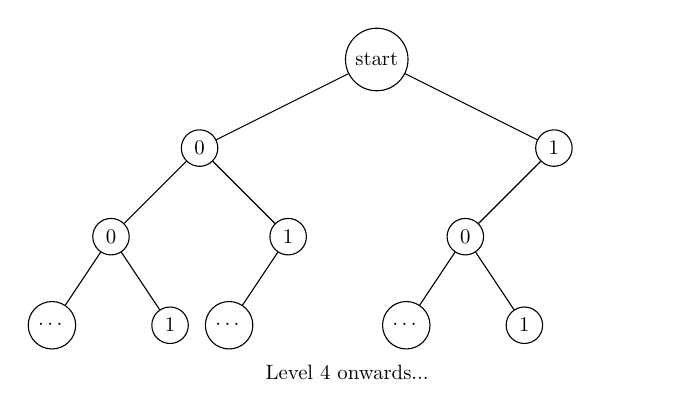
\begin{tikzpicture}[level/.style={sibling distance=60mm/#1}, scale=0.75, every node/.style={scale=0.75}]
                \node [circle, draw] (start) {start}
                child {node [circle, draw] (a) {$0$}
                    child {node [circle, draw] (b) {$0$}
                        child {node [circle, draw] (d) {$\cdots$}}
                        child {node [circle, draw] (e) {$1$}}
                    }
                    child {node [circle, draw] (c) {$1$}
                        child {node [circle, draw] (f) {$\cdots$}}
                        child {node [circle, draw=none] (g) {$\quad$} edge from parent[draw=none]}
                    }
                }
                child {node [circle, draw] (j) {$1$}
                    child {node [circle, draw] (k) {$0$}
                        child {node [circle, draw] (m) {$\cdots$}}
                        child {node [circle, draw] (n) {$1$}
                        }
                    }
                    child {node [circle] {$\quad$} edge from parent[draw=none]  % Placeholder to maintain structure
                    }
                };
                
        
                % Indicating that the pattern continues
                \node at ($(g) + (0,-0.8)$) {Level 4 onwards...};
            \end{tikzpicture}
            \caption{Binary Tree Illustrating Counting of Binary Strings with Repeated 1s}
        \end{figure}

        \begin{yap}
            FIBONACCI WHY ARE YOU HERE?? HMMM?? Also, if you look at the sequence of possible lists of each length, take length 4, the answer would be 8. It's easy if you only checked strings of length 4 to say that there are half of the total possible strings, $2^4$.
        \end{yap}

\newpage
\setcounter{subsection}{2}
    \subsection{Selections and Arrangements}

        \subsubsection{Permutations}

            \begin{definition}
                We define a \textit{permutation} as where we choose $r$ people from $n$ choices, where order matters! $$nPr = P(n,r)$$
            \end{definition}
    
            \begin{example}
                In how many distinct ways can $n$ people line up? Such that $n,n-1,n-2\dots,1$ ($n$ slots). 
            \end{example}
    
            \sol{
                $n!$
            }
    
            \begin{example}
                What if we want to have $r$ people from $n$ line up such that $(r\leq n)$. Such that $n,n-1,n-2,\dots,n-r+1$ ($r$ slots).
            \end{example}
    
            \sol{
                $\displaystyle \frac{n!}{(n-r)!}$ \\  
        }

        \vspace{0.5cm}

            \begin{definition}
                What if order does not matter? $$\frac{nPr}{r!} = nCr = \frac{n!}{(n-r)!r!}$$
            \end{definition}
    
            \begin{example}
                We want to choose 5 people from 32 (32 being the amount of people in the class). How many possible combinations are there?
            \end{example}
    
            \sol{
                $\displaystyle \binom{32}{5} = 201,376$.
            }
            
            \begin{example}
                An urn contains 12 numbered marbles, $1,2\dots,12$. 5 are selected. How many distinct outcomes are possible? Answer the following:
                \begin{itemize}
                    \item With or without replacement
                \end{itemize}
            \end{example}

            \sol{
                Consider the following chooses:
                \begin{itemize}
                    \item With replacement, order matters. $12^5$. 
                    \item With replacement, order does not matter.* 
                    \item Without replacement, order matters. $_{12}P_5 = \frac{12!}{7!}$ 
                    \item Without replacement, order does not matter. $\displaystyle \binom{12}{5} = \frac{12!}{7!\cdot 5!}$
                \end{itemize}
                * We must use the Binomial Theorem: $$(a+b)^n = \sum_{r=0}^{n}\binom{n}{r}a^{r}b^{n-r}$$
            }

            \noindent Consider the following solution for $(x+3)^5$ with the bimodal theorem: $$\binom{5}{5}x^5\cdot 3^0+\binom{5}{4}x^4\cdot 3 + \binom{5}{3}x^3\cdot 3^2 + \binom{5}{2}x^2\cdot 3^3 + \binom{5}{1}x^1\cdot 3^4 + \binom{5}{0}x^0\cdot 3^5$$ \\

            \noindent Note that $\binom{5}{4}$ and $\binom{5}{1}$ will always produce the same answer because $\binom{n}{n-r}$

\newpage
\setcounter{subsection}{4}
    \subsection{Counting In Algorithms}
            \begin{lstlisting}
    x = 4
    for i in [1,2,...,n]:
        x = x + 1

    # If n = 3, what is the final value of x?

    i = 1, x = 5 # There are three additions.
    i = 2, x = 6
    i = 3, x = 7

    # In general, the line x = x + 1 runs n times total.

    for i in [1,2,3,...,n]:
        c = c + i + 5 + b
        for j in [1,2,3,...n]:
            a = a + b + 1

    # Note the outer for loop is n additions, and the inner loop is 2n additions.

    for i in [1,2,3,...,n]:
        for j in [i, i + 1,..., n]:
            a = a + b + 1

    # Total: 2 * (n(n+1)) / 2 = n ** 2 + n additions. 
            \end{lstlisting}

        \subsubsection{Big-O Classes (From handout p.3)}

            $n^3 + 3n^2 - 8n + 1 \in \Theta(n^3)$ \\

            Look at the highest power or piece that grows the fastest. \textbf{Important}: Constants do not matter. \\

            \noindent $(n^3 + 4n)(\log_2(n) + 5) \in \Theta(n^3\log_2(n))$ \\

            Multiply the largest growing terms.

        
            
\newpage
    
%------------------------------------------------------------------------------


\section{Algorithms}
    \begin{definition}
        \textbf{Terms}: \\
        \underline{Pre condition}: Initial input/state. \\
        \underline{Post condition}: Final state/output.
    \end{definition}

    \begin{yap}
        blah blah if you're familiar with algorithms its like a computer program, its what we really tell the computer what to do.
    \end{yap}

    \begin{definition}
        \textit{Linear Search}: Given a list of integers and a target value, return \underline{True}, if target is in the list, \underline{False} if otherwise.
    \end{definition}

    Say, for the list, $lst$, consider $[x_0,x_1,\dots,x_{n-1}]$. \\
    For the target value, $t$, we want to know two things: \begin{enumerate}
        \item Is $t$ in the list?
        \item Where is it?
    \end{enumerate}
    \textbf{Pseudo-code}:
    \begin{lstlisting}
    i = 0
    x_n = t # Sentinal value 
    while t < > x_i: # "While t is not equal to x_i..."
        i = i + 1
    if i = n:
        print ('Not there')
    else:
        print('Found at i')

    i = 0
    x_n = t # Sentinal value 
    while t < > x_i: # "While t is not equal to x_i..."
    if i = n:
        print ('Not there')
    else:
        print('Found at i')
    i = i + 1

    # Now it checks index 0 ? before why would we have it as 0 if we just skip to 1 anyway before our comparison
    \end{lstlisting}

    The maximum number of additions with this algorithm is $n$. \\
    \indent And the minimum number of additions is 0.
    
    \begin{yap}
        When reasoning with post-conditions, we can use pre-conditions that we know are true in order to simplify the algorithm.
    \end{yap}

    \begin{table}[ht]
            \centering
            \begin{tabular}{c|c}
                $\text{Post-condition Claim}$ & $\text{Pre-condition claim}$ \\
                \hline
                $x_i = t$ & $t \in list$ \\
            \end{tabular}
            \caption{something about conditions matching}
            \label{Bottom Up A(n)}
    \end{table}
    \textit{Post-condition claim}: $x_i = t$ \\
    \textit{Pre-condition claim}: $t \in lst$

    We want to prove this using proof by induction. (Note: The base case is always that the loop is not running.) \\

    \underline{Base Case}: \\
    $t = x_0$.\\

    \underline{Inductive Hypothesis}: \\
    Assume $x_i = t$ if $t \in lst$, assume $x_i$ if $t \text{ is later (?)}$, and assume $t$ appears only once in the list. \\

    \underline{Inductive Step}: \\
    We need to prove that $x_{i + 1} = t$ if $t$ is at $i + 1$, and $x_{i + 1} = t$, if $t$ is not at $i + 1$. \\
    Cases: \begin{enumerate}
        \item $t$ is at $i + 1$: then $x_i$ is not equal to $t$
    \end{enumerate}

    \begin{yap}
        Apparently coders don't need to prove their code works if they believe their code is sound in logic and would not be cost effective to prove.
    \end{yap}

    \begin{enumerate}
        \item What is the biggest value in a list?
    \end{enumerate}

    \begin{lstlisting}
    big = x_0
    for x_n in list
        if x_n > big
            big = x_n
    print(big)
    \end{lstlisting}

    The maximum and minimum number of comparisons with this algorithm is $n-1$. \\

    \begin{table}[ht]
            \centering
            \begin{tabular}{c|c}
                $\text{Post-condition Claim}$ & $\text{Pre-condition claim}$ \\
                \hline
                $\forall x_i \in list, big > x_i$ & $n \geq 1$ \\
            \end{tabular}
            \caption{something about conditions matching}
            \label{Bottom Up A(n)}
    \end{table}

    We want to prove this by induction. (Note: The base case is always that the loop is not running.) \\

    \underline{Base Case}: $i=n \rightarrow n=1$\\
    big = $x_0$ \\
    $x_0 \geq x_0$ is true. \\

    \underline{Inductive Hypothesis}: \\
    $i \leq n, \forall x_i \in$ list, big $\geq x_i$ \\

    \underline{Inductive Step}: \\
    We need to prove that $x_{i + 1} = t$ if $t$ is at $i + 1$, and $x_{i + 1} = t$, if $t$ is not at $i + 1$. \\
    Cases: \begin{enumerate}
        \item $t$ is at $i + 1$: then $x_i$ is not equal to $t$
    \end{enumerate}


    \subsection{Greedy Algorithms}

    \begin{definition}
        \textit{Prim's Algorithm} finds a minimal spanning tree in an edge-weighted graph. Where a \textit{Spanning Tree} is a tree that uses only the edges (and of course, the vertices) of the main graph.
    \end{definition}
    \noindent To make a spanning tree: Make the original blank graph (just the vertices), throw edges in, and never make a circuit. 

    \noindent A \textit{minimal} spanning tree is one that gives the total, smallest weight of the edges that are on the graph. That is, if $A--B$ is weight 5, and $A--C$ is weight 3, and $B--C$ is weight 1, how can you choose all edges that are of the smallest total weight? 

    \subsection{Traveling Salesperson Problem}
    Given a connected weighted graph, find a minimal cost Hamilton circuit (use each vertex one time).

\subsection{Algorithms review}
    \begin{definition}
        Linear Search: iterate through list, one element at a time. $\theta (n)$
    \end{definition}
    \begin{definition}
        Binary Search: Given a sorted list, find a target value.
    \end{definition}
    Unsorted list: $[7,1,8,2,4,9]$, linear search, 6 iterations. \\
    Sorted list: $[1,2,4,7,8,9]$, binary search, 3 iterations or in general, $log_2n$.
    


%------------------------------------------------------------------------------
%------------------------------------------------------------------------------
%------------------------------------------------------------------------------
%------------------------------------------------------------------------------

\end{document}
